\documentclass[a4paper,11pt]{article}
\usepackage{titling}
\usepackage{graphics}
\usepackage[italian]{babel}\selectlanguage{italian}
\usepackage{graphicx}
\usepackage{titlesec}
\usepackage{enumitem}
\usepackage{hyperref}
\usepackage{csquotes}
\usepackage{wrapfig}
\usepackage{float}
\usepackage{array}
\usepackage{caption}
\usepackage{booktabs}
\usepackage{url}
\usepackage{longtable}
%% \usepackage{todonotes}
\usepackage{listings}
\usepackage{imakeidx}
\usepackage{minted}
\usepackage{setspace}
\usepackage{hyperref}
\hypersetup{
    colorlinks=true,
    linkcolor=blue,
    filecolor=magenta,
    urlcolor=cyan,
    pdftitle={Overleaf Example},
    pdfpagemode=FullScreen,
    }
\urlstyle{same}
\usepackage[
backend=biber,
style=numeric,
sorting=ydnt
]{biblatex}
\addbibresource{./ref.bib}

\setminted{
    linenos=true,
    autogobble,
    breaklines,
    frame=single
}
\usepackage{mathptmx}
\usepackage{geometry}
 \geometry{
 a4paper,
 left=35mm
 }
\onehalfspacing
\newenvironment{longlisting}{\captionsetup{type=figure}}{}

\title{Blockchain e IoT \\ tracciabilità e controlli automatici}
\author{Paola Guarasci}
\date{Settembre 2024}
\makeindex
\begin{document}

\begin{titlepage}
  \begin{center}
    \textbf{\LARGE Universit\`a della Calabria}\\
    \textbf{Dipartimento di Matematica e Informatica}\\
    \vskip 6pt
    \hrule
    \vskip 8pt
    
\includegraphics{./img/logo_unical.png}
    \vskip 8pt
    \textbf{Corso di Laurea Magistrale in Informatica}
    \vskip 32pt
    Tesi di Laurea

    \vskip 70pt
      { \huge \bfseries Blockchain e IoT \\ tranciabilità e controlli automatici}\\[0.4cm]
    \vskip 150pt

    \begin{tabular}{p{8cm}p{8cm}}
      Relatore:           & Candidata:       \\
      Prof.~Mario Alviano & Paola Guarasci   \\
                          & Matricola 231847 \\
    \end{tabular}

    \vskip 76pt
    \hrule
    \vskip 5pt
    Anno Accademico 2023/2024
    \vfill
  \end{center}

\end{titlepage}
\clearpage
\tableofcontents
\clearpage
\begin{abstract}
  Lorem ipsum...
\end{abstract}
\section{Introduzione}
\section{Background}

\subsection{Digital Twin}

\subsection{Blockchain}
La tecnologia dei registri distribuiti, distribuited ledger tecnlogy o DLT, consenta di utilizzare dati digitali in modo distribuito, condiviso e sincronizzato. Non necessita di una entità centrale. La blockchain identifica un particolare tipo di registro distribuito.


\paragraph{Scalabilità}
% Il concetto di scalabilita' all'interno delle blockchain

\paragraph{Il trilemma delle blockchain}

% Non si possono avere tutte insieme!

\begin{figure}[h!]
  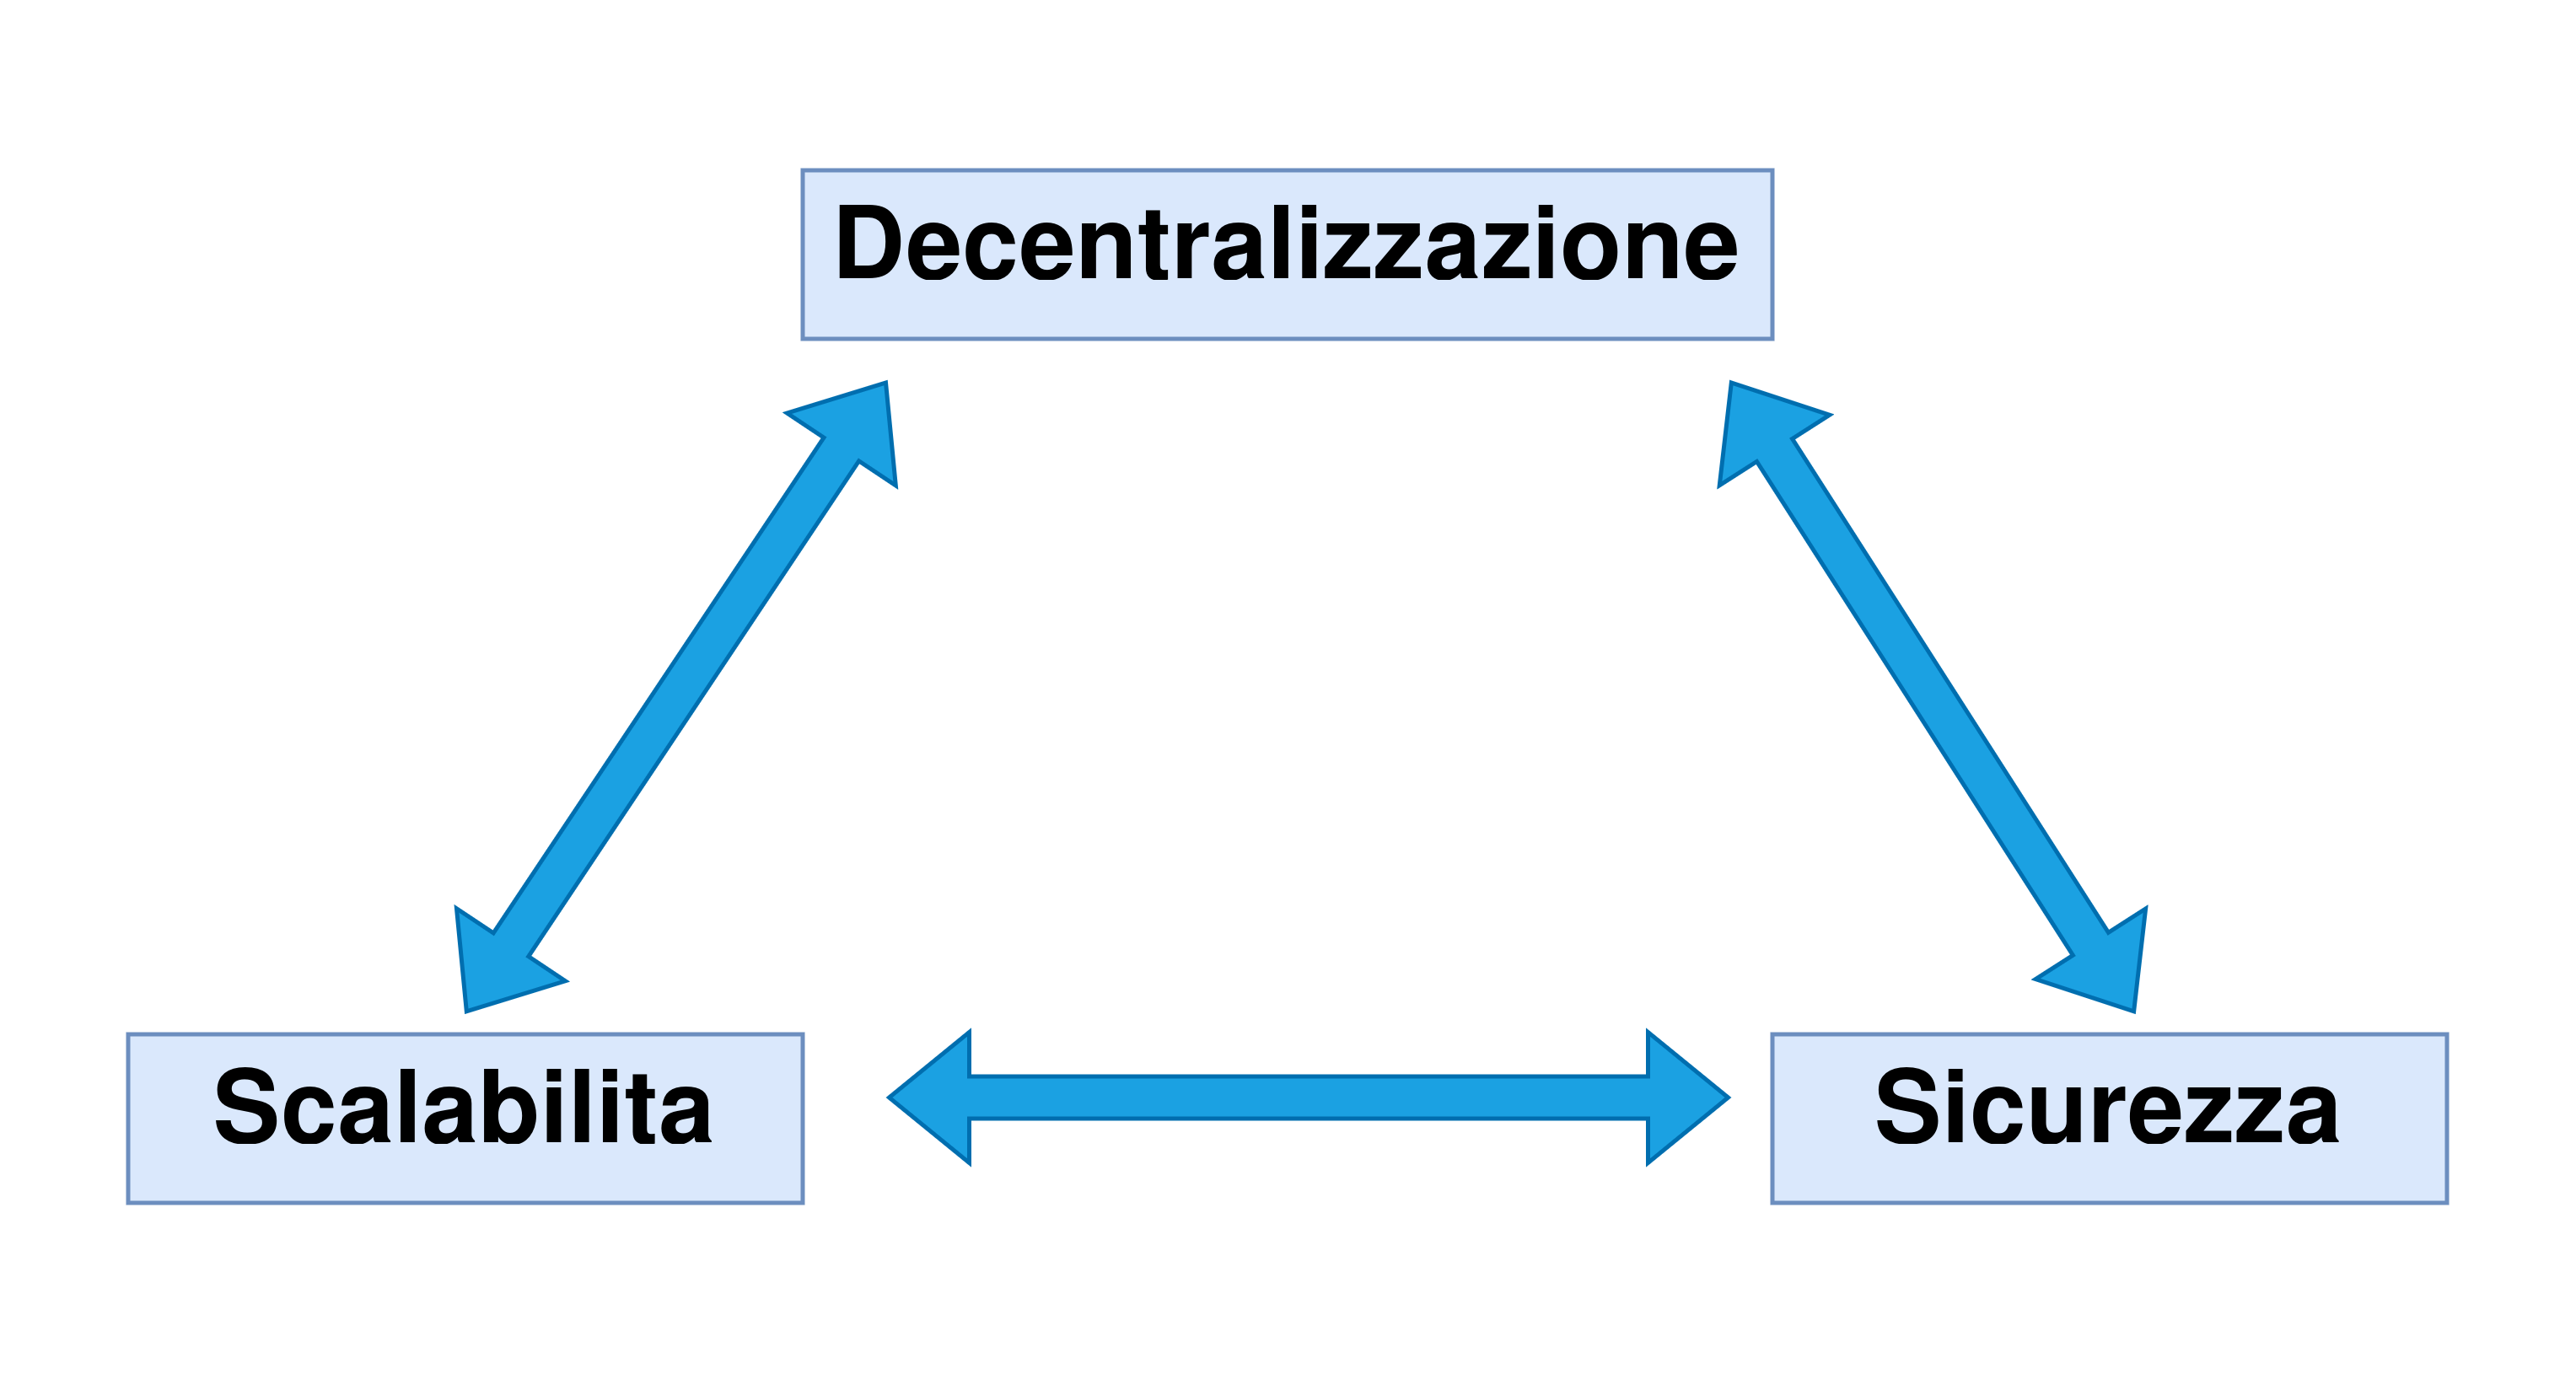
\includegraphics[width=1\linewidth]{img/trilemma.png}
  \caption{Il trilemma della blockchain}
  \label{fig:trilemma}
\end{figure}

\paragraph{Layer1 e Layer2}
Le reti blockchain principali hanno definite \textit{layer 1} e rappresentalo reti che funzionano da sole. Le reti layer 2, di contro, sono reti che si pongo, utilizzando diverse metodologie, come sovrastuttura rispetto alla layer 1 che espandono. Di fatto rappresentano appunto delle espansioni delle reti principali. Il motibvo

\paragraph{Algoritmi di consenso}
\paragraph{Permiossionless e Permissioned}
\paragraph{Ethereum}
\paragraph{Polygon}
\paragraph{Tools}

\subsection{ASP}

\subsection{Concetti di Tracciabilità e di Filiera}

\section{Analisi dello stato dell’arte della tecnologia blockchain applicata alle supplychain}
\section{Definizione di un caso d’uso}
Il caso d'uso che si vuole analizzare riguarda la tracciabilità di un prodotto inserito nella filiera agroalimentare. Un esempio potrebbe essere la tracciabilità di un ipotetico prodotto surgelato, ad esempio un minestrone, di cui si vuole tenere traccia, in modo immutabile dalla raccolta delle materie prime fino alla vendita finale.






















% TODO:


% inserire un confronto tra le varie chian e indicare perché è stata scelta poligon













\subsection{Progettazione}
Il software presenta un'architettura client-server con un componente principale, il server, ed un componente secondario, il client. Il client è un client non corrisponde del tutto alla definizione di client stupido. Si avvicina infatti più alla definizione di fat client.
Il sistema implementa un'architettura a tre livelli in cui il livello di presentazione è stratificato. I livelli di un'applicazione a tre tier sono:
\begin{itemize}
  \item Livello di presentazione
  \item Livello applicazione (business logic)
  \item Livello dati
\end{itemize}

\begin{figure}[H]
  \includegraphics[width=1\linewidth]{example-image-a}
  \caption{Architettura}
  \label{fig:architettura}
\end{figure}

% (immagine architettura)
% (descrizione dei livelli)


Si è deciso di utilizzare una struttura monolitica e non a microservizi.La comunicazione tra componente server e componente client avviene tramite RestAPI. La costruzione di api rest implica alcuni vincoli architeturali \cite{restfulapiRESTArchitectural}

- Bisogna definire un'interfaccia uniforme
- Avere un'architettura client server in cui un componente chiede risorse (client) e un altro le espone (server)
- Il server è senza stato ovvero il server non ha memoria delle connessioni precedenti
- Per le richieste in lettura si può prevedere un meccanismo di cache in cui il server propone gli stessi contenuti. Bisogna prevedere anche criteri di aggiornamento e invalidamento dei contenuti in cache.
- Implementare un sistema a livelli, in cui il client si connette ad un servizio senza conoscere l'architettura interna
- Codice on demand (opzionale) quando necessario, oltre alle risorse statiche, è possibile inserire del codice eseguibile nella risposta del server

L'autenticazione utilizza il protocollo OAuth2 ed un'istanza di Keycloak come authentication server. \cite{ietf6749OAuth}

\begin{figure}[H]
  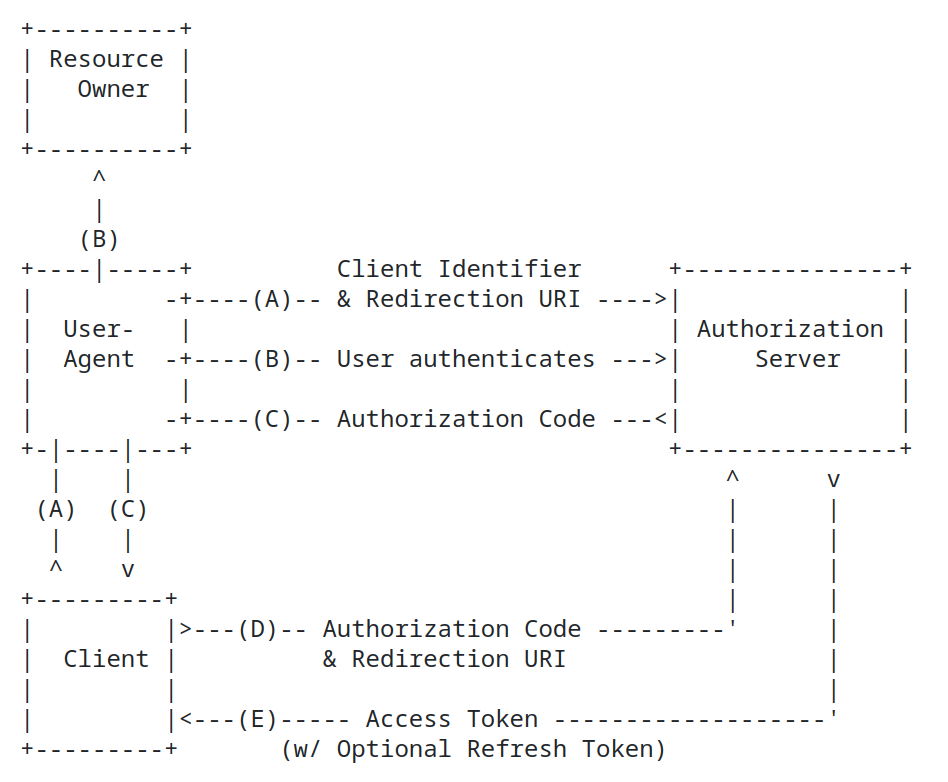
\includegraphics[width=1\linewidth]{img/image-1.png}
  \caption{Authorization Flow in OAuth2 \cite{ietf6749OAuth}}
  \label{fig:authorizationoauth2}
\end{figure}

Lo stack tecnologico utilizzato comprende
Sono stati presi in esame diversi framework per la componente server. In ambito NodeJS sono stati presi in considerazione NestJS ed Express.

\paragraph{Descrizione di Nest}
Nest (NestJS) is a framework for building efficient, scalable Node.js server-side applications. It uses progressive JavaScript, is built with and fully supports TypeScript (yet still enables developers to code in pure JavaScript) and combines elements of OOP (Object Oriented Programming), FP (Functional Programming), and FRP (Functional Reactive Programming). [...] In recent years, thanks to Node.js, JavaScript has become the "lingua franca" of the web for both front and backend applications. This has given rise to awesome projects like Angular, React and Vue, which improve developer productivity and enable the creation of fast, testable, and extensible frontend applications. However, while plenty of superb libraries, helpers, and tools exist for Node (and server-side JavaScript), none of them effectively solve the main problem of - Architecture. Nest provides an out-of-the-box application architecture which allows developers and teams to create highly testable, scalable, loosely coupled, and easily maintainable applications. The architecture is heavily inspired by Angular. \cite{nestjsDocumentationNestJS}

\paragraph{Descrizione di Express}

Express è un framework per applicazioni web Node.js flessibile e leggero che fornisce una serie di funzioni avanzate per le applicazioni web e per dispositivi mobili. Con una miriade di metodi di utilità HTTP e middleware a disposizione, la creazione di un'API affidabile è un processo facile e veloce. Express fornisce uno strato sottile di funzionalità di base per le applicazioni web, senza nascondere le funzioni Node.js. \cite{expressjsExpressFramework}

\paragraph{Descrizione di Spring e Spring Boot}

Spring è un framework java. Spring Boot è una sua estensione. Tipicamente si utilizzano insieme, è ormai difficile immaginare di usare Spring senza Spring Boot. Spring si basa sull'inversione del controllo e sull'injection delle dipendenze. Il principio di design di inversione del controllo, IoC, descrive quelle situazioni in cui un componente software applicativo riceve il controllo da parte di un componente di libreria e non il contrario come avviene in una programmazione procedurare tradizionale in cui il software applicativo utilizza (e controlla) le componenti di libreria. In questo contesto si inserisce l'iniezione delle dipendenze che è un altro aspetto fondamentale del framework Spring, che elimina dall'applicazione ogni logica di inizializzazione. È il framework stesso che quando necessario inietta un riferimento all'implementazione del servizio richiesto. \cite{wikipediaInversioneControllo}

Spring Boot crea applicazioni Spring standalone, con un application server embedded a scelta tra Tomcat o Jetty.
Spring Boot semplifica il processo di sviluppo perché abbraccia lo stile Convention-over-configuration ed utilizza configurazioni standard la dove il programmatore non ha definito una configurazione personalizzata per quel particolare aspetto del software in svilupo. Esistono difatti moduli di spring boot che fanno da "starter" per i diversi moduli di spring. La configurazione, quando è necessaria, non deve in ogni caso essere redatta in XML. \cite{wikipediaSpringBoot}

\paragraph{Scelta del framework e considerazioni personali }

Express.JS si è rivelato eccessivamente granulare e di basso livello per gli scopi del progetto. NestJS e Spring, sebbene molto simili tra di loro, soprattutto su alcuni aspetti di design quali l'inversione del controllo e l'injection delle dipendenze, che sono concetti che si possono ritrovare in entrambi i framework, utilizzano due ecosistemi differenti, il primo NodeJS ed il secondo Java. Si è scelto di utilizzare Java per poter utilizzare a pieno i vantaggi di una programmazione orientata agli oggetti in un ambiente multithread. NodeJs ha una natura asincrona e dalla documentazione di node.js \cite{nodedontblock} si legge

In a one-thread-per-client system like Apache, each pending client is assigned its own thread. If a thread handling one client blocks, the operating system will interrupt it and give another client a turn. The operating system thus ensures that clients that require a small amount of work are not penalized by clients that require more work. Because Node.js handles many clients with few threads, if a thread blocks handling one client's request, then pending client requests may not get a turn until the thread finishes its callback or task. The fair treatment of clients is thus the responsibility of your application. This means that you shouldn't do too much work for any client in any single callback or task. This is part of why Node.js can scale well, but it also means that you are responsible for ensuring fair scheduling. The next sections talk about how to ensure fair scheduling for the Event Loop and for the Worker Pool.


Il server utilizza il pattern repository ed altri pattern in maniera più o meno esplicita

Gestione delle transazioni
% Una transazione è un'operazione atomica che avviene all'interno di un'applicazione server o su una base di dati. Tipicamente le transazioni hanno
% vedi https://www.baeldung.com/spring-programmatic-transaction-management#transaction-template
% TRANSAZIONI HIBERNATE e TRANSAZIONI DI SPRING
% https://docs.jboss.org/hibernate/stable/orm/userguide/html_single/Hibernate_User_Guide.html#transactions

LATO AUTENTICAZIONE


LATO CLIENT

I framework lato client presi in esame sono Vue.js, Angular e React.
I dati di diffusione di questi framework li pongono ai primi tre posti di una ipotetica classifica basata sull'utilizzo misurato in numero di repository pubblici. Se si guarda all'utilizzo al primo posto troviamo React seguito da Vue e poi da Angular. Riguardo l'awareness (conoscenza) invece Angular passsa in prima posizione, Vue mantiene il secondo posto e React scivola in terza posizione \cite{stateofjsStateJavaScript}.

Vue.js

Vue is a JavaScript framework for building user interfaces. It builds on top of standard HTML, CSS, and JavaScript and provides a declarative, component-based programming model that helps you efficiently develop user interfaces of any complexity. [...] Vue is a framework and ecosystem that covers most of the common features needed in frontend development. But the web is extremely diverse - the things we build on the web may vary drastically in form and scale. With that in mind, Vue is designed to be flexible and incrementally adoptable. [...] Despite the flexibility, the core knowledge about how Vue works is shared across all these use cases. Even if you are just a beginner now, the knowledge gained along the way will stay useful as you grow to tackle more ambitious goals in the future. If you are a veteran, you can pick the optimal way to leverage Vue based on the problems you are trying to solve, while retaining the same productivity. This is why we call Vue "The Progressive Framework": it's a framework that can grow with you and adapt to your needs. \cite{vuejsVuejs}

React

React (noto anche come React.js o ReactJS) è una libreria open-source, front-end, JavaScript per la creazione di interfacce utente. È mantenuto da Meta (già Facebook) e da una comunità di singoli sviluppatori e aziende.
React può essere utilizzato come base nello sviluppo di applicazioni a pagina singola ma è utilizzabile anche su mobile tramite React Native, una libreria sempre sviluppata da Meta che tramuta i componenti React in componenti nativi (iOS e Android). Tuttavia, React si occupa solo del rendering dei dati sul DOM, pertanto la creazione di applicazioni React richiede generalmente l'uso di librerie aggiuntive per lo state management e il routing. Redux e React Router sono i rispettivi esempi di tali librerie. A questo fine è possibile utilizzare anche dei framework terzi, come ad esempio Next.js. \cite{wikipediaReactweb}

Angular.JS

Angular is a web framework that empowers developers to build fast, reliable applications. Maintained by a dedicated team at Google, Angular provides a broad suite of tools, APIs, and libraries to simplify and streamline your development workflow. Angular gives you a solid platform on which to build fast, reliable applications that scale with both the size of your team and the size of your codebase. \cite{angularAngular}

Scelta e motivazioni

\subsubsection{Analisi dei requisiti}

I requisiti funzionali di alto livello sono i seguenti:

\begin{itemize}
  \item Ogni utente registrato opera per conto di una compagnia
  \item Un utente registrato deve poter creare tipologie di prodotto, indicando un template di ricetta e di processo produttivo
  \item Un utente registrato deve poter creare un nuovo lotto di prodotti di una determinata tipologia, con una ricetta, uno o più documenti allegati ed indicando le fasi di produzione di cui si vuole tenere traccia
  \item Un utente registrato deve poter trasferire (in modo atomico) un lotto di prodotti ad un'altra compagnia
  \item Un utente registrato deve poter inserire un documento e notarizzarlo
  \item Un utente registrato deve poter accedere in lettura ai dati di notarizzazione dei documenti caricati
  \item Un utente registrato deve poter trasferire con accettazione un lotto di prodotti ad un'altra compagnia
  \item Un utente registrato deve poter rifiutare il trasferimento con accettazione di un lotto trasferito alla compagnia per cui opera
  \item Un utente registrato deve poter accettare il trasferimento con accettazione di un lotto trasferito alla compagnia per cui opera
  \item Un utente registrato deve poter annullare il trasferimento con accettazione di un lotto disposto dalla sua compagnia
  \item Un utente registrato deve poter visualizzare le informazioni di tracciamento relative ai lotti di cui è in possesso la sua compagnia
  \item Un utente registrato deve poter avviare una spedizione per i trasferimenti conclusi e avviati dalla sua compagnia
  \item Un utente registrato deve poter visualizzare informazioni telemetriche delle spedizioni in corso
  \item Un utente non registrato deve poter visualizzare le informazioni pubbliche di tracciamento di un lotto di produzione
\end{itemize}
s
I requisiti non funzionali sono applicabili alla quasi totalità dei sistemi, ovvero:

\begin{itemize}
  \item Sicurezza: Il sistema deve essere protetto da accessi non autorizzati.
  \item Performance: Il sistema deve essere in grado di gestire il numero richiesto di utenti senza alcun degrado delle prestazioni.
  \item Scalabilità: Il sistema deve essere in grado di aumentare o diminuire in base alle esigenze.
  \item Disponibilità: Il sistema deve essere disponibile quando necessario.
  \item Manutenzione: Il sistema deve essere di facile manutenzione e aggiornamento.
  \item Portabilità: Il sistema deve essere in grado di funzionare su piattaforme diverse con modifiche minime.
  \item Affidabilità: Il sistema deve essere affidabile e soddisfare i requisiti dell'utente.
  \item Usabilità: Il sistema deve essere facile da usare e da capire.
  \item Compatibilità: Il sistema deve essere compatibile con altri sistemi.
  \item Compliance: Il sistema deve essere conforme a tutte le leggi e i regolamenti applicabili.
\end{itemize}

\subsubsection{Casi d'uso}
Sono stati individuati i seguenti casi d'uso:

\begin{itemize}
  \item CU1: Registrazione di un tipo di prodotto
  \item CU2: Registrazione di un lotto prodotto
  \item CU3: Tracciamento di un lotto (utente registrato)
  \item CU4: Tracciamento di un lotto (utente non registrato)
  \item CU5: Trasferimento di un lotto (atomico) [INCLUDE trasferimento]
  \item CU6: Trasferimento di un lotto (con accettazione) [INCLUDE trasferimento]
  \item CU7: Accettazione di un trasferimento
  \item CU8: Ritiro di un trasferimento
  \item CU9: Rifiuto di un trasferimento
  \item CU10: Notarizzazione di un documento
  \item CU11: Avvio di una spedizione
  \item CU12: Registrazione di un utente
  \item CU13: Login di un utente
\end{itemize}

Specifiche dei casi d'uso:

\begin{table}[H]
  \centering
  \begin{tabular}{|m{2cm}|m{10.5cm}|}
    \hline
    \multicolumn{2}{|c|}{\textbf{Registrazione di un tipo di prodotto}}                \\ \hline
    \multicolumn{1}{|l|}{\textbf{ID}}              & CU1                               \\ \hline
    \multicolumn{1}{|l|}{\textbf{Attori}}          & Utente registrato                 \\ \hline
    \multicolumn{1}{|l|}{\textbf{Precondizioni}}   & Utente autenticato in piattaforma \\ \hline
    \multicolumn{1}{|l|}{\textbf{Sequenza}}        &
    \begin{itemize}
      \item Il caso d'uso inizia quando l'utente clicca su "crea nuovo tipo di prodotto"
      \item L'utente inserisce un nome
      \item Se l'utente clicca su "aggiungi ricetta"
            \begin{itemize}
              \item Il sistema avvia il caso d'uso CU1a
            \end{itemize}
      \item Se l'utente clicca su salva
            \begin{itemize}
              \item il sistema salva il nuovo tipo di prodotto
            \end{itemize}
      \item Se l'utente clicca su cancella
            \begin{itemize}
              \item il sistema annulla l'inserimento e non salva nessun dato
            \end{itemize}
    \end{itemize}  \\ \hline
    \multicolumn{1}{|l|}{\textbf{Post-condizioni}} & --                                \\ \hline
  \end{tabular}
  \caption{Caso d'uso 1 - Registrazione di un tipo di prodotto}
  \label{cu:CU1}
\end{table}

\begin{table}[H]
  \centering
  \begin{tabular}{|m{2cm}|m{10.5cm}|}
    \hline
    \multicolumn{2}{|c|}{\textbf{Creazione di una ricetta (estende CU1 Registrazione di un tipo di prodotto)}}                                                      \\ \hline
    \multicolumn{1}{|l|}{\textbf{ID}}              & CU1a                                                                                                           \\ \hline
    \multicolumn{1}{|l|}{\textbf{Attori}}          & Utente registrato                                                                                              \\ \hline
    \multicolumn{1}{|l|}{\textbf{Precondizioni}}   & Utente autenticato in piattaforma                                                                              \\ \hline
    \multicolumn{1}{|l|}{\textbf{Sequenza}}        &

    \begin{itemize}
      \item Il caso d'uso inizia quando l'utente clicca su "aggiungi ricetta" durante la creazione di un tipo di prodotto
      \item L'utente seleziona un tipo di prodotto tra quelli già registrati e la quantità percentuale desiderata.
      \item Il sistema memorizza temporaneamente i dati inseriti
      \item Il sistema consente di inserire un nuovo item di ricetta
      \item Il sistema consente di rimuovere ogni item inserito
      \item Se l'utente clicca su aggiungi item
            \begin{itemize}
              \item vai al passo 2
            \end{itemize}
      \item Se l'utente clicca su rimuovi item
            \begin{itemize}
              \item il sistema elimina l'item selezionatos
              \item vai al passo 1
            \end{itemize}
      \item Se l'utente clicca su cancella
            \begin{itemize}
              \item il sistema annulla l'inserimento della ricetta, termina il caso d'uso e prosegue il caso d'uso CU1
            \end{itemize}
      \item Se l'utente clicca su salva
            \begin{itemize}
              \item il sistema salva temporaneamente la ricetta, termina il caso d'uso e prosegue il caso d'uso CU1
            \end{itemize}
    \end{itemize}

    \\ \hline
    \multicolumn{1}{|l|}{\textbf{Post-condizioni}} & Se l'utente ha cliccato su salva la ricetta è stata salva correttamente nei dati temporanei del caso d'uso CU1 \\ \hline
  \end{tabular}
  \caption{Caso d'uso 1a - Creazione di una ricetta (estende CU1 Registrazione di un tipo di prodotto) }
  \label{cu:CU1a}
\end{table}

\begin{table}[H]
  \centering
  \begin{tabular}{|m{2cm}|m{10.5cm}|}
    \hline
    \multicolumn{2}{|c|}{\textbf{Registrazione di un lotto prodotto)}}                                                                                                     \\ \hline
    \multicolumn{1}{|l|}{\textbf{ID}}              & CU2                                                                                                                   \\ \hline
    \multicolumn{1}{|l|}{\textbf{Attori}}          & Utente registrato                                                                                                     \\ \hline
    \multicolumn{1}{|l|}{\textbf{Precondizioni}}   & L'utente è autenticato in piattaforma e la compagnia per cui opera l'utente ha almeno un tipo di prodotto registrato. \\ \hline
    \multicolumn{1}{|l|}{\textbf{Sequenza}}        &
    \begin{itemize}
      \item Il caso d'uso inizia quando l'utente clicca su "Inserisci nuovo lotto di prodotto"
      \item L'utente inserisce identificativo, descrizione e quantità del lotto
      \item L'utente seleziona il tipo di prodotto tra i tipi di prodotto già inseriti in piattaforma
      \item Il sistema carica il processo produttivo del tipo di prodotto selezionato.
      \item L'utente può selezionare uno o più step del processo produttivo del tipo selezionato
      \item Se il tipo di prodotto ha una ricetta

            %   \begin{itemize}
            %       \item il sistema consente all'utente di selezionare uno o più item di ricetta da inserire nella ricetta specifica del lotto che si sta creando
            %     \item L'utente inserisce le coordinate geografiche della produzione
            %     \item Se l'utente clicca su salva
            %   \begin{itemize}
            %   \item Se il prodotto ha una ricetta
            %     \begin{itemize}
            %     \item Il sistema verifica che siano presenti sufficienti risorse per la creazione del lotto (ASP)
            %       \begin{itemize}
            %       \item Se le risorse non sono sufficienti
            %         \begin{itemize}
            %         \item Il sistema notifica l'utente
            %         \end{itemize}
            %       \end{itemize}
            %       \begin{itemize}
            %       \item Se le risorse sono sufficienti
            %         \begin{itemize}
            %           \item Il sistema seleziona i lotti di materie prime da utilizzare nella creazione del lotto (ASP) (usando la ricetta)
            %           \item Il sistema aggiorna le quantità dei lotti selezionati (usando la ricetta)
            %           \item Il sistema crea il lotto di prodotto
            %           \item Il sistema notarizza la creazione del lotto di prodotto
            %         \end{itemize}
            %       \end{itemize}
            %     \end{itemize}
            %   \end{itemize}
    \end{itemize}
    \\ \hline
    \multicolumn{1}{|l|}{\textbf{Post-condizioni}} &
    \begin{itemize}
      \item Il lotto di prodotto è stato creato
      \item Le quantità delle materie prime sono state correttamente aggiornate
      \item La creazione del lotto di prodotto è stata notarizzata
      \item L'utente può visualizzare la notarizzazione nell'elenco notarizzazioni
    \end{itemize}
    \\ \hline
  \end{tabular}
  \caption{Caso d'uso 2 - Registrazione di un lotto di prodotto}
  \label{cu:CU2}
\end{table}

\begin{table}[H]
  \centering
  \begin{tabular}{|m{2cm}|m{10.5cm}|}
    \hline
    \multicolumn{2}{|c|}{\textbf{Tracciamento di un lotto (utente registrato)}}                                                                                             \\ \hline
    \multicolumn{1}{|l|}{\textbf{ID}}              & CU3                                                                                                                    \\ \hline
    \multicolumn{1}{|l|}{\textbf{Attori}}          & Utente registrato                                                                                                      \\ \hline
    \multicolumn{1}{|l|}{\textbf{Precondizioni}}   & L'utente è autenticato in piattaforma e la compagnia per cui opera l'utente ha almeno un lotto di prodotto registrato. \\ \hline
    \multicolumn{1}{|l|}{\textbf{Sequenza}}        &

    \begin{itemize}
      \item Il caso d'uso inizia quando l'utente clicca su "Traccia" di un lotto di produzione
      \item Il sistema fornisce informazioni di tracciamento combinando la lista di materie prime, i singoli processi di ogni materia prima e le informazioni di notarizzazione con processi e notarizzazione del prodotto principale
      \item Se l'utente seleziona Notarizza in uno qualunque degli step visibili inizia il caso d'uso CU3a\ref{cu:CU3a}
    \end{itemize}
    \\ \hline
    \multicolumn{1}{|l|}{\textbf{Post-condizioni}} & --                                                                                                                     \\ \hline
  \end{tabular}
  \caption{Caso d'uso 3 - Tracciamento di un lotto (utente registrato}
  \label{cu:CU3}
\end{table}

\begin{table}[H]
  \centering
  \begin{tabular}{|m{2cm}|m{10.5cm}|}
    \hline
    \multicolumn{2}{|c|}{\textbf{ Notarizzazione di uno step di processo (Estende: CU3\ref{cu:CU3} )}}                                                                                                                                                                                   \\ \hline
    \multicolumn{1}{|l|}{\textbf{ID}}              & CU3a                                                                                                                                                                                                                                \\ \hline
    \multicolumn{1}{|l|}{\textbf{Attori}}          & Utente registrato                                                                                                                                                                                                                   \\ \hline
    \multicolumn{1}{|l|}{\textbf{Precondizioni}}   & L'utente è autenticato in piattaforma, la compagnia per cui opera l'utente ha almeno un lotto di prodotto registrato e l'utente sta visualizzando le informazioni di tracciamento del lotto di produzione prodotto dalla compagnia. \\ \hline
    \multicolumn{1}{|l|}{\textbf{Sequenza}}        &
    \begin{itemize}

      \item Il caso d'uso inizia quando l'utente seleziona "Notarizza" di uno step visualizzato nel tracciamento di un lotto di produzione (CU3\ref{cu:CU3})
      \item Il sistema salva su un registro immutabile una descrizione dello step
      \item Il sistema attende l'operazione di salvataggio
      \item Il sistema allega allo step che si sta notarizzando un riferimento univoco all'operazione di salvataggio nel registro immutabile

    \end{itemize}
    \\ \hline
    \multicolumn{1}{|l|}{\textbf{Post-condizioni}} & L'identificativo univoco è visualizzato in CU3\ref{cu:CU3}                                                                                                                                                                          \\ \hline
  \end{tabular}
  \caption{Caso d'uso 3a - Notarizzazione di uno step di processo}
  \label{cu:CU3a}
\end{table}


\begin{table}[H]
  \centering
  \begin{tabular}{|m{2cm}|m{10.5cm}|}
    \hline
    \multicolumn{2}{|c|}{\textbf{Tracciamento di un lotto (utente non registrato))}} \\ \hline
    \multicolumn{1}{|l|}{\textbf{ID}}              & CU4                             \\ \hline
    \multicolumn{1}{|l|}{\textbf{Attori}}          & Utente non registrato           \\ \hline
    \multicolumn{1}{|l|}{\textbf{Precondizioni}}   & TODO                            \\ \hline
    \multicolumn{1}{|l|}{\textbf{Sequenza}}        & TODO                            \\ \hline
    \multicolumn{1}{|l|}{\textbf{Post-condizioni}} & TODO                            \\ \hline
  \end{tabular}
  \caption{Caso d'uso 4 - Tracciamento di un lotto (utente registrato}
  \label{cu:CU4}
\end{table}


\begin{table}[H]
  \centering
  \begin{tabular}{|m{2cm}|m{10.5cm}|}
    \hline
    \multicolumn{2}{|c|}{\textbf{Trasferimento di un lotto (atomico) [INCLUDE trasferimento])}}                  \\ \hline
    \multicolumn{1}{|l|}{\textbf{ID}}                 & CU5                                                      \\ \hline
    \multicolumn{1}{|l|}{\textbf{Attori}}             & Utente registrato che opera per conto di una compagnia A \\ \hline
    \multicolumn{1}{|l|}{\textbf{Precondizioni}}      &
    \begin{itemize}
      \item L'utente è autenticato in piattaforma
      \item Esiste una compagnia B registrata in piattaforma
      \item La compagnia A ha un lotto di prodotto registrato
    \end{itemize}
    \\ \hline
    \multicolumn{1}{|l|}{\textbf{Sequenza}}           &

    \begin{itemize}
      \item Il caso d'uso inizia quando l'utente seleziona un lotto e clicca su "Trasferisci"
      \item L'utente seleziona la compagnia destinataria, la quantità di prodotto da inviare e sceglie il tipo di trasferimento atomico
      \item Il sistema controlla che i dati inseriti siano corretti
      \item Se la quantità di prodotto è sufficiente allora C6x
      \item Se la quantità di prodotto non è sufficiente
      \item Il sistema avvisa l'utente
      \item Il caso d'uso termina
    \end{itemize}

    \\ \hline
    \multicolumn{1}{|l|}{\textbf{Post-condizioni}}    &
    \begin{itemize}
      \item Se C6x
            \begin{itemize}
              \item Il lotto creato è visibile alla compagnia destinataria
              \item Il lotto di partenza ha la quantità aggiornata
            \end{itemize}
      \item Altrimenti
            \begin{itemize}
              \item Il lotto di partenza non ha subito variazioni
              \item La compagnia destinataria non visualizza nuovi lotti
            \end{itemize}
    \end{itemize}
    \\ \hline
    \multicolumn{1}{|l|}{\textbf{Flusso alternativo}} &

    Il caso d'uso può ripetersi finché l'utente non seleziona una quantità di risorse che ha effettivamente a disposizione

    \\ \hline
  \end{tabular}
  \caption{Caso d'uso 5 - Trasferimento di un lotto (atomico) [INCLUDE trasferimento] }
  \label{cu:CU5}
\end{table}


\begin{table}[H]
  \centering
  \begin{tabular}{|m{2cm}|m{10.5cm}|}
    \hline
    \multicolumn{2}{|c|}{\textbf{Trasferimento di un lotto (atomico) [INCLUDE trasferimento])}} \\ \hline
    \multicolumn{1}{|l|}{\textbf{ID}}              & CU6x                                       \\ \hline
    \multicolumn{1}{|l|}{\textbf{Attori}}          & --                                         \\ \hline
    \multicolumn{1}{|l|}{\textbf{Precondizioni}}   & --                                         \\ \hline
    \multicolumn{1}{|l|}{\textbf{Sequenza}}        &

    \begin{itemize}
      \item Il caso d'uso inizia quando al sistema arriva una richiesta di trasferimento di un lotto o porzione di esso dal proprietario attuale verso un nuovo proprietario
      \item Il sistema crea un nuovo lotto a partere dalle informazioni del lotto originale e lo assegna alla compagnia destinataria
      \item Il sistema aggiorna la quantità di prodotto nel lotto originale
      \item Il sistema rende immutabile il trasferimento (notarizzazione)
      \item Il sistema allega la notarizzazione al trasferimento

    \end{itemize}

    \\ \hline
    \multicolumn{1}{|l|}{\textbf{Post-condizioni}} &
    --
    \\ \hline
  \end{tabular}
  \caption{Caso d'uso 6x - Trasferimento}
  \label{cu:CU6x}
\end{table}



\begin{longtable}{|p{2cm}|p{13cm}|}
  \multicolumn{2}{c}{\textbf{Trasferimento di un lotto (con accettazione) [INCLUDE trasferimento]}} \\ \hline
  \textbf{ID}              & CU6                                                                    \\ \hline
  \textbf{Attori}          &

  \begin{itemize}
    \item Utente A registrato che opera per conto di una compagnia A
    \item Utente B registrato che opera per conto di una compagnia B
  \end{itemize}

  \\ \hline
  \textbf{Precondizioni}   &

  \begin{itemize}
    \item L'utente A è autenticato in piattaforma
    \item L'utente B è autenticato in piattaforma
    \item La compagnia A ha un lotto di prodotto registrato
  \end{itemize}

  \\ \hline
  \textbf{Sequenza}        &

  \begin{itemize}
    \item Il caso d'uso inizia quando l'utente seleziona un lotto e clicca su "Trasferisci"
    \item L'utente seleziona la compagnia destinataria, la quantità di prodotto da inviare e sceglie il tipo di trasferimento con accettazione
    \item Il sistema controlla che i dati inseriti siano corretti
    \item Se la quantità di prodotto non è sufficiente
          \begin{itemize}
            \item Il sistema avvisa l'utente
          \end{itemize}
    \item Se la quantità di prodotto è sufficiente
          \begin{itemize}
            \item Il sistema blocca la risorsa da trasferire
            \item Il sistema notifica all'utente B la presenza di un trasferimento in ingresso (casi d'uso CU7 e CU9)
            \item Il sistema rende annullabile trasferimento da parte dell'utente A (caso d'uso CU8)
            \item Se si verifica CU7 allora CU6x \ref{cu:CU6x}
            \item Se si verifica CU9 o CU8
                  \begin{itemize}
                    \item Il sistema ripristina la quantità di prodotto bloccata nel lotto originale
                    \item Il caso d'uso termina
                  \end{itemize}
          \end{itemize}
  \end{itemize}

  \\ \hline
  \textbf{Post-condizioni} &
  \begin{itemize}
    \item Se C6x \ref{cu:CU6x}
          \begin{itemize}
            \item Il lotto creato è visibile alla compagnia destinataria
            \item Il lotto di partenza ha la quantità aggiornata
          \end{itemize}
    \item Altrimenti
          \begin{itemize}
            \item Il lotto di partenza non ha subito variazioni
            \item La compagnia destinataria non visualizza nuovi lotti
          \end{itemize}
  \end{itemize}
  \\ \hline
  \caption{Caso d'uso 6 - Trasferimento di un lotto con accettazione [INCLUDE C6x \ref{cu:CU6x} Trasferimento]}
  \label{cu:CU6}
\end{longtable}




\begin{table}[H]
  \centering
  \begin{tabular}{|m{2cm}|m{10.5cm}|}
    \hline
    \multicolumn{2}{|c|}{\textbf{Accettazione di un trasferimento)}}           \\ \hline
    \multicolumn{1}{|l|}{\textbf{ID}}              & CU7                       \\ \hline
    \multicolumn{1}{|l|}{\textbf{Attori}}          &

    Utente registrato che opera per conto della compagnia destinataria del trasferimento

    \\ \hline
    \multicolumn{1}{|l|}{\textbf{Precondizioni}}   &

    La compagnia per cui opera l'utente registrato ha un trasferimento in ingresso di tipo "con accettazione"

    \\ \hline
    \multicolumn{1}{|l|}{\textbf{Sequenza}}        &

    \begin{itemize}
      \item Il caso d'uso inizia quando l'utente visualizza la lista di trasferimenti della compagnia per cui opera
      \item L'utente seleziona accetta un trasferimento di tipo con accettazione e
      \item il sistema notifica l'accettazione alla compagnia mittente
    \end{itemize}

    \\ \hline
    \multicolumn{1}{|l|}{\textbf{Post-condizioni}} & Inizia CU6x \ref{cu:CU6x} \\ \hline
  \end{tabular}
  \caption{Caso d'uso 7 - Accettazione di un trasferimento}
  \label{cu:CU7}
\end{table}

\begin{table}[H]
  \centering
  \begin{tabular}{|m{2cm}|m{10.5cm}|}
    \hline
    \multicolumn{2}{|c|}{\textbf{Ritiro di un trasferimento)}} \\ \hline
    \multicolumn{1}{|l|}{\textbf{ID}}              & CU8       \\ \hline
    \multicolumn{1}{|l|}{\textbf{Attori}}          &

    Utente registrato che opera per conto della compagnia mittente del trasferimento

    \\ \hline
    \multicolumn{1}{|l|}{\textbf{Precondizioni}}   &
    \begin{itemize}
      \item La compagnia per cui opera l'utente registrato ha un trasferimento in ingresso di tipo "con accettazione"
      \item Il trasferimento non è stato ancora accettato dalla compagnia destinataria
    \end{itemize}
    \\ \hline
    \multicolumn{1}{|l|}{\textbf{Sequenza}}        &

    \begin{itemize}
      \item Il caso d'uso inizia quando l'utente visualizza la lista di trasferimenti della compagnia per cui opera
      \item L'utente seleziona Ritira un trasferimento di tipo con accettazione
      \item Il sistema notifica il ritiro alla compagnia destinataria
      \item Il sistema aggiorna la quantità del lotto originario
    \end{itemize}

    \\ \hline
    \multicolumn{1}{|l|}{\textbf{Post-condizioni}} & --        \\ \hline
  \end{tabular}
  \caption{Caso d'uso 8 - Ritiro di un trasferimento}
  \label{cu:CU8}
\end{table}


\begin{table}[H]
  \centering
  \begin{tabular}{|m{2cm}|m{10.5cm}|}
    \hline
    \multicolumn{2}{|c|}{\textbf{Rifiuto di un trasferimento)}} \\ \hline
    \multicolumn{1}{|l|}{\textbf{ID}}              & CU9        \\ \hline
    \multicolumn{1}{|l|}{\textbf{Attori}}          &

    Utente registrato che opera per conto della compagnia destinataria del trasferimento

    \\ \hline
    \multicolumn{1}{|l|}{\textbf{Precondizioni}}   &
    La compagnia per cui opera l'utente registrato ha un trasferimento in ingresso di tipo "con accettazione"
    \\ \hline
    \multicolumn{1}{|l|}{\textbf{Sequenza}}        &

    \begin{itemize}
      \item Il caso d'uso inizia quando l'utente visualizza la lista di trasferimenti della compagnia per cui opera
      \item L'utente seleziona rifiuta un trasferimento di tipo con accettazione
      \item Il sistema notifica il rifiuto alla compagnia mittente
      \item Il sistema aggiorna la quantità del lotto originario
    \end{itemize}

    \\ \hline
    \multicolumn{1}{|l|}{\textbf{Post-condizioni}} & --         \\ \hline
  \end{tabular}
  \caption{Caso d'uso 9 - Rifiuto di un trasferimento}
  \label{cu:CU9}
\end{table}

\begin{table}[H]
  \centering
  \begin{tabular}{|m{2cm}|m{10.5cm}|}
    \hline
    \multicolumn{2}{|c|}{\textbf{Notarizzazione di un documento)}} \\ \hline
    \multicolumn{1}{|l|}{\textbf{ID}}              & CU10          \\ \hline
    \multicolumn{1}{|l|}{\textbf{Attori}}          &

    Utente registrato in piattaforma

    \\ \hline
    \multicolumn{1}{|l|}{\textbf{Precondizioni}}   &
    Utente autenticato e in possesso di un documento in formato pdf o jpg/png da notarizzare
    \\ \hline
    \multicolumn{1}{|l|}{\textbf{Sequenza}}        &

    \begin{itemize}
      \item Il caso d'uso inizia quando l'utente seleziona "Carica documento"
      \item L'utente sceglie dal suo dispositivo un documento nei formati consentiti (pdf, jpg o png)
      \item L'utente clicca su carica
      \item Il sistema effettua il caricamento della risorsa
      \item Il sistema salva un'impronta digitale della risorsa all'interno del registro immutabile
      \item Il sistema memorizza un riferimento univoco al salvataggio del punto precedente
      \item Il sistema restituisce un indirizzo web per la verifica della transazione sul registro immutabile
    \end{itemize}

    \\ \hline
    \multicolumn{1}{|l|}{\textbf{Post-condizioni}} &

    \begin{itemize}
      \item La risorsa è disponibile per il download
      \item L'operazione di notarizzazione è pubblicamente verificabile
    \end{itemize}

    \\ \hline
  \end{tabular}
  \caption{Caso d'uso 10 - Notarizzazione di un documento}
  \label{cu:CU10}
\end{table}

\begin{table}[H]
  \centering
  \begin{tabular}{|m{2cm}|m{10.5cm}|}
    \hline
    \multicolumn{2}{|c|}{\textbf{Avvio di una spedizione)}} \\ \hline
    \multicolumn{1}{|l|}{\textbf{ID}}              & CU11   \\ \hline
    \multicolumn{1}{|l|}{\textbf{Attori}}          &

    Utente registrato in piattaforma

    \\ \hline
    \multicolumn{1}{|l|}{\textbf{Precondizioni}}   &
    Utente autenticato in piattaforma, esiste una transazione completata (accettata o atomica) avviata dalla compagnia per cui opera l'utente e non è stato ancora disposto il trasferimento per la transazione
    \\ \hline
    \multicolumn{1}{|l|}{\textbf{Sequenza}}        &

    \begin{itemize}
      \item Il caso d'uso inizia quando l'utente visualizza la lista delle transazioni
      \item Se l'utente seleziona una transazione completata e clicca su "Invia"
            \begin{itemize}
              \item Il sistema cerca un camion disponibile
              \item Se ci sono camion disponibili
                    \begin{itemize}
                      \item il sistema associa il camion al lotto oggetto della transazione
                      \item il sistema aggiorna periodicamente le letture dei sensori associati al camion
                      \item il sistema salva in modo immutabile le letture dei sensori
                    \end{itemize}
              \item Se non ci sono camion disponibili
                    \begin{itemize}
                      \item Il sistema notifica un errore
                    \end{itemize}
            \end{itemize}
    \end{itemize}

    \\ \hline
    \multicolumn{1}{|l|}{\textbf{Post-condizioni}} &

    Si può vedere la lista delle letture dei sensori associati al camion

    \\ \hline
  \end{tabular}
  \caption{Caso d'uso 11 - Avvio di una spedizione }
  \label{cu:CU11}
\end{table}


\begin{figure}[H]
  \includegraphics[width=1\linewidth]{example-image-b}
  \caption{Diagramma dei casi d'uso}
  \label{fig:diagrammacasi}
\end{figure}


\subsubsection{Persistenza}

La piattaforma che si sta sviluppando utilizza un sistema di gestione della persistenza che è di tipo relazionale. Nello specifico utilizza il database managment system MariaDB con Hibernate come strato di comunicazione con l'applicazione. Hibernate implementa le API Java Persistence (JPA).

Hibernate è un ORM, un Object/Relational Mapping, un modulo software che gestisce la persistenza in contesti in cui si utilizza una base di dati relazionale.

Hibernate not only takes care of the mapping from Java classes to database tables (and from Java data types to SQL data types), but also provides data query and retrieval facilities. It can significantly reduce development time otherwise spent with manual data handling in SQL and JDBC. Hibernate’s design goal is to relieve the developer from 95\% of common data persistence-related programming tasks by eliminating the need for manual, hand-crafted data processing using SQL and JDBC. However, unlike many other persistence solutions, Hibernate does not hide the power of SQL from you and guarantees that your investment in relational technology and knowledge is as valid as always. \cite{jbossHibernateUser}

\begin{figure}[H]
  \centering
  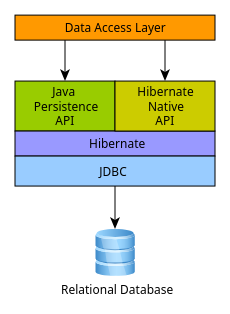
\includegraphics[width=0.4\linewidth]{img/image-3.png}
  \caption{Dove si colloca Hibernate? \cite{jbossHibernateUserArch}}
  \label{fig:architetturahibernate}
\end{figure}


\subsubsection{Definizione del modello di dominio}\label{modellodominio}

La definizione di un modello di dominio a partire dai concetti principali che caratterizzano il modello di business individuato per l'applicazione.
Sono stati individuati i seguenti concetti propri dell'ambito applicativo.
Entità e attributi:

\begin{itemize}
  \item Batch
        \begin{itemize}
          \item Descrizione: Il lotto rappresenta un'unità di produzione di un particolare tipo di prodotto, in una determinata quantità.
          \item Attributi: id, batchId, quantity, isFinal, productionDate, processType
        \end{itemize}
  \item ProductType
        \begin{itemize}
          \item Descrizione: Il tipo di prodotto è un generico prodotto inteso come l'astrazione, la generalizzazione, di lotti di produzione.
          \item Attributi: id, name, unity, state
        \end{itemize}
  \item Recipe (di ProductType)
        \begin{itemize}
          \item Descrizione: Lista di ingredienti che compongono in generico prodotto. E' il modello da utilizzare quando si materializza la ricetta vera e propria durante la produzione di un lotto.
          \item Attributi: id, note, recipeRow
        \end{itemize}
  \item RecipeBatch (di Batch)
        \begin{itemize}
          \item Descrizione: Lista di ingredienti effettivamente utilizzati nella produzione di un lotto di produzione.
          \item Attributi: id, note, recipeRow
        \end{itemize}
  \item ProductionProcess (di ProductType)
        \begin{itemize}
          \item Descrizione: Lista di passi da seguire durante il processo produttivo del tipo cui l'entità si riferisce
          \item Attributi: id, note, steps
        \end{itemize}
  \item ProductionProcessBatch (di Batch)
        \begin{itemize}
          \item Descrizione: Lista di passi da seguire durante il processo produttivo del tipo cui l'entità si riferisce
          \item Attributi: id, note, steps
        \end{itemize}
  \item Document
        \begin{itemize}
          \item Descrizione: Risorsa che rappresenta un certificato, un'analisi o una generica attestazione da legare al lotto di produzione
          \item Attributi: id, title, description, link, path
        \end{itemize}
  \item Notarize
        \begin{itemize}
          \item Descrizione: Entità che modella il concetto di notarizzazione di una qualunque risorsa all'interno della piattaforma. Consente di raccogliere insieme una o più transazioni reali sulla blockchain che hanno un legame logico tra di loro.
          \item Attributi: id, hash, notarizedAt, data
        \end{itemize}
  \item Transfer
        \begin{itemize}
          \item Descrizione: Rappresentazione del trasferimento di un Batch o porzione di esso tra due Company registrate in piattaforma, si in modo atomico che con accettazione.
          \item Attributi: id, type, status, oldBatchID, newBatchID, quantity, unity, companySenderID, companySenderUsername, companyRecipientID, companyRecipientUsername, transferDateStart, lastUpdate
        \end{itemize}
  \item Transport
        \begin{itemize}
          \item Descrizione:
          \item Attributi: id, truckId, batchId, dateStart, dateEnd, location, companyFrom, companyTo
        \end{itemize}
  \item Truck:
        \begin{itemize}
          \item Descrizione: Modellazione del mezzo fisico (camion) che effettua il trasporto, ipotetico luogo dove si collocano i sensori che si vuole utilizzare
          \item Attributi: id, lastSensorsUpdate
        \end{itemize}
  \item UserInfo
        \begin{itemize}
          \item Descrizione: Entità che rappresenta l'utente in piattaforma. Ha un riferimento al'auth server di Oauth2s.
          \item Attributi: id, username, keycloakUsername, keycloakId, email, firstName, lastName
        \end{itemize}
  \item Company
        \begin{itemize}
          \item Descrizione: Modellazione dell'azienda che produce lotto di prodotti e che effettua operazioni su di essi in piattaforma.
          \item Attributi: id, name
        \end{itemize}
  \item ChainTransaction
        \begin{itemize}
          \item Descrizione: Rappresenta la transazione sulla blockchain
          \item Attributi: id, txId
        \end{itemize}
  \item Location
        \begin{itemize}
          \item Descrizione:
          \item Attributi:
        \end{itemize}
\end{itemize}

Relazioni:

\begin{itemize}
  \item Company - Batch:
        \begin{itemize}
          \item Cardinalità: uno a molti con partecipazione opzionale
          \item Descrizione: Ogni Company può avere da 0 a n Batch prodotti. Ogni Batch ha una ed una sola Company che lo produce.
          \item Ruolo: Produttore
        \end{itemize}
  \item Company - Batch:
        \begin{itemize}
          \item Cardinalità: uno a molti con partecipazione opzionale
          \item Descrizione: Ogni Company può avere da 0 a n Batch detenuti. Ogni Batch ha una ed una sola Company che lo detiene.
          \item Ruolo: Proprietario
        \end{itemize}
  \item ProductType - Batch:
        \begin{itemize}
          \item Cardinalità: uno a molti con partecipazione opzionale
          \item Descrizione: Ogni ProductType può avere uno o più Batch che lo materializza. Un Batch ha esattamente un ProductType.
        \end{itemize}
  \item Location - Batch;
        \begin{itemize}
          \item Cardinalità: uno a molti con partecipazione opzionale
          \item Descrizione: Ogni Location può essere il luogo di produzione di zero o più Batch. Un Batch ha esattamente una Location.
        \end{itemize}
  \item Document - Batch;
        \begin{itemize}
          \item Cardinalità: molti a molti con partecipazione opzionale
          \item Descrizione: Ogni Document puà essere legato a più Batch, ogni Batch può avere collegati zero o più Document.
        \end{itemize}
  \item RecipeBatch - Batch:
        \begin{itemize}
          \item Cardinalità:
          \item Descrizione:
        \end{itemize}
  \item ProductionProcessBatch - Batch:
        \begin{itemize}
          \item Cardinalità:
          \item Descrizione:
        \end{itemize}
  \item ProductType - Company:
        \begin{itemize}
          \item Cardinalità: Molti a molti
          \item Descrizione: Ogni tipo di prodotto può essere legato ad una o più Company ed ogni Company può utilizzare uno o più tipi di prodotto
        \end{itemize}
  \item UserInfo - Company:
        \begin{itemize}
          \item Cardinalità: uno a molti con partecipazione obbligatoria
          \item Descrizione: Un utente (UserInfo) ha esattamente una compagnia (Company) collegata. Ogni compagnia (Company) ha almeno un utente collegato.
        \end{itemize}
  \item Notarize - Document:
        \begin{itemize}
          \item Cardinalità: uno ad uno con partecipazione opzionale
          \item Descrizione: Ogni Document ha alpiù una notarizzazione ed ogni Notarize può avere alpiù un Document
        \end{itemize}
  \item Company - Document:
        \begin{itemize}
          \item Cardinalità: uno a molti con partecipazione opzionale
          \item Descrizione: Ogni Document da riferimento ad esattamente una Company. Una Company puoò avere zero o più Document collegati.
        \end{itemize}
  \item Company - Notarize:
        \begin{itemize}
          \item Cardinalità: uno a molti con partecipazione obbligatoria
          \item Descrizione: Una Notarize ha esattamente una Company che l'ha creata ed una Company può creare zero o più Notarize.
        \end{itemize}
  \item ChainTransaction - Notarize:
        \begin{itemize}
          \item Cardinalità: uno a molti con partecipazione obbligatoria
          \item Descrizione: Una Notarize ha almeno una ChainTransaction (transazione effettiva sulla blockchain). Ogni ChainTransaction fa riferimento ad una sola Notarize.
        \end{itemize}
  \item ProductionStep - ProductionProcess
        \begin{itemize}
          \item Cardinalità: uno a molti con partecipazione obbligatoria
          \item Descrizione: Un processo produttivo di tipo (ProductionProcess) ha almeno uno step di produzione di tipo (ProductionStep). Ogni step (ProductionStep) fa parte di un singolo processo produttivo (ProductionProcess).
        \end{itemize}
  \item ProductionStepBatch - ProductionProcessBatch
        \begin{itemize}
          \item Cardinalità: uno a molti con partecipazione obbligatoria
          \item Descrizione: Un processo produttivo di lotto (ProductionProcessBatch) ha almeno uno step di produzione di lotto (ProductionStepBatch). Ogni step (ProductionStepBatch) fa parte di un singolo processo produttivo (ProductionProcessBatch).
        \end{itemize}
  \item ProductionStepBatch - Notarize
        \begin{itemize}
          \item Cardinalità: uno ad uno con partecipazione opzionale
          \item Descrizione: Ogni processo produttivo di lotto (ProductionStepBatch) può avere al più un atto di notarizzazione (Notarize).
        \end{itemize}
  \item Recipe - ProductType:
        \begin{itemize}
          \item Cardinalità:
          \item Descrizione:
        \end{itemize}
  \item ProductionProcess - ProductType:
        \begin{itemize}
          \item Cardinalità:
          \item Descrizione:
        \end{itemize}
  \item Recipe - RecipeRow:
        \begin{itemize}
          \item Cardinalità: uno a molti con partecipazione obligatoria
          \item Descrizione: Ogni ricetta di tipo (Recipe) ha almeno un ingrediente \\ di tipo(RecipeRow).
        \end{itemize}
  \item RecipeBatch - RecipeRowBatch:
        \begin{itemize}
          \item Cardinalità: uno a molti con partecipazione obligatoria
          \item Descrizione: Ogni ricetta di lotto (RecipeBatch) ha almeno un ingrediente di lotto (RecipeRowBatch).
        \end{itemize}
  \item RecipeRow - ProductType:
        \begin{itemize}
          \item Cardinalità: uno a molti con partecipazione obbligatoria
          \item Descrizione: Ogni riga di ricetta di tipo (RecipeRow) si riferisce ad esattamente un tipo di prodotto (ProductType). Ogni ProductType può fare parte di zero o più ricette di tipo.
        \end{itemize}
  \item RecipeRowBatch - Batch
        \begin{itemize}
          \item Cardinalità: uno a molti con partecipazione obbligatoria
          \item Descrizione: Ogni riga di ricetta di lotto (RecipeRowBatch) si riferisce ad esattamente un lotto di prodotto (Batch). Ogni Batch può fare parte di zero o più ricette di lotto.
        \end{itemize}
  \item SensorsLog - Notarize
        \begin{itemize}
          \item Cardinalità: uno a molti con partecipazione opzionale
          \item Descrizione: Gruppi di item di log dei sensori (SensorsLog) possono fare riferimento ad uno stesso item di notarizzazione (Notarize) se sono stati raggruppati e notarizzati nello stesso momento, per esempio per letture ravvicinate nel tempo.
        \end{itemize}
  \item ChainTransaction - Transfer
        \begin{itemize}
          \item Cardinalità: uno a molti con partecipazione opzionale
          \item Descrizione: Ogni trasferimento di lotti (Transfer) si riferisce ad una o più transazioni effettive sulla chain (ChainTransaction). Per esempio, il tipo con accettazione prevede tre transazioni.
        \end{itemize}
  \item Truck - Company
        \begin{itemize}
          \item Cardinalità: uno a molti
          \item Descrizione: Ogni Truck fa riferimento ad una sola Company
        \end{itemize}
  \item Truck - MyDt
        \begin{itemize}
          \item Cardinalità: uno a molti
          \item Descrizione: Ogni Truck ha una lista di gemelli digitali collegati
        \end{itemize}
\end{itemize}


%% --------- SCHEMA classi ------------------

\begin{figure}[H]
  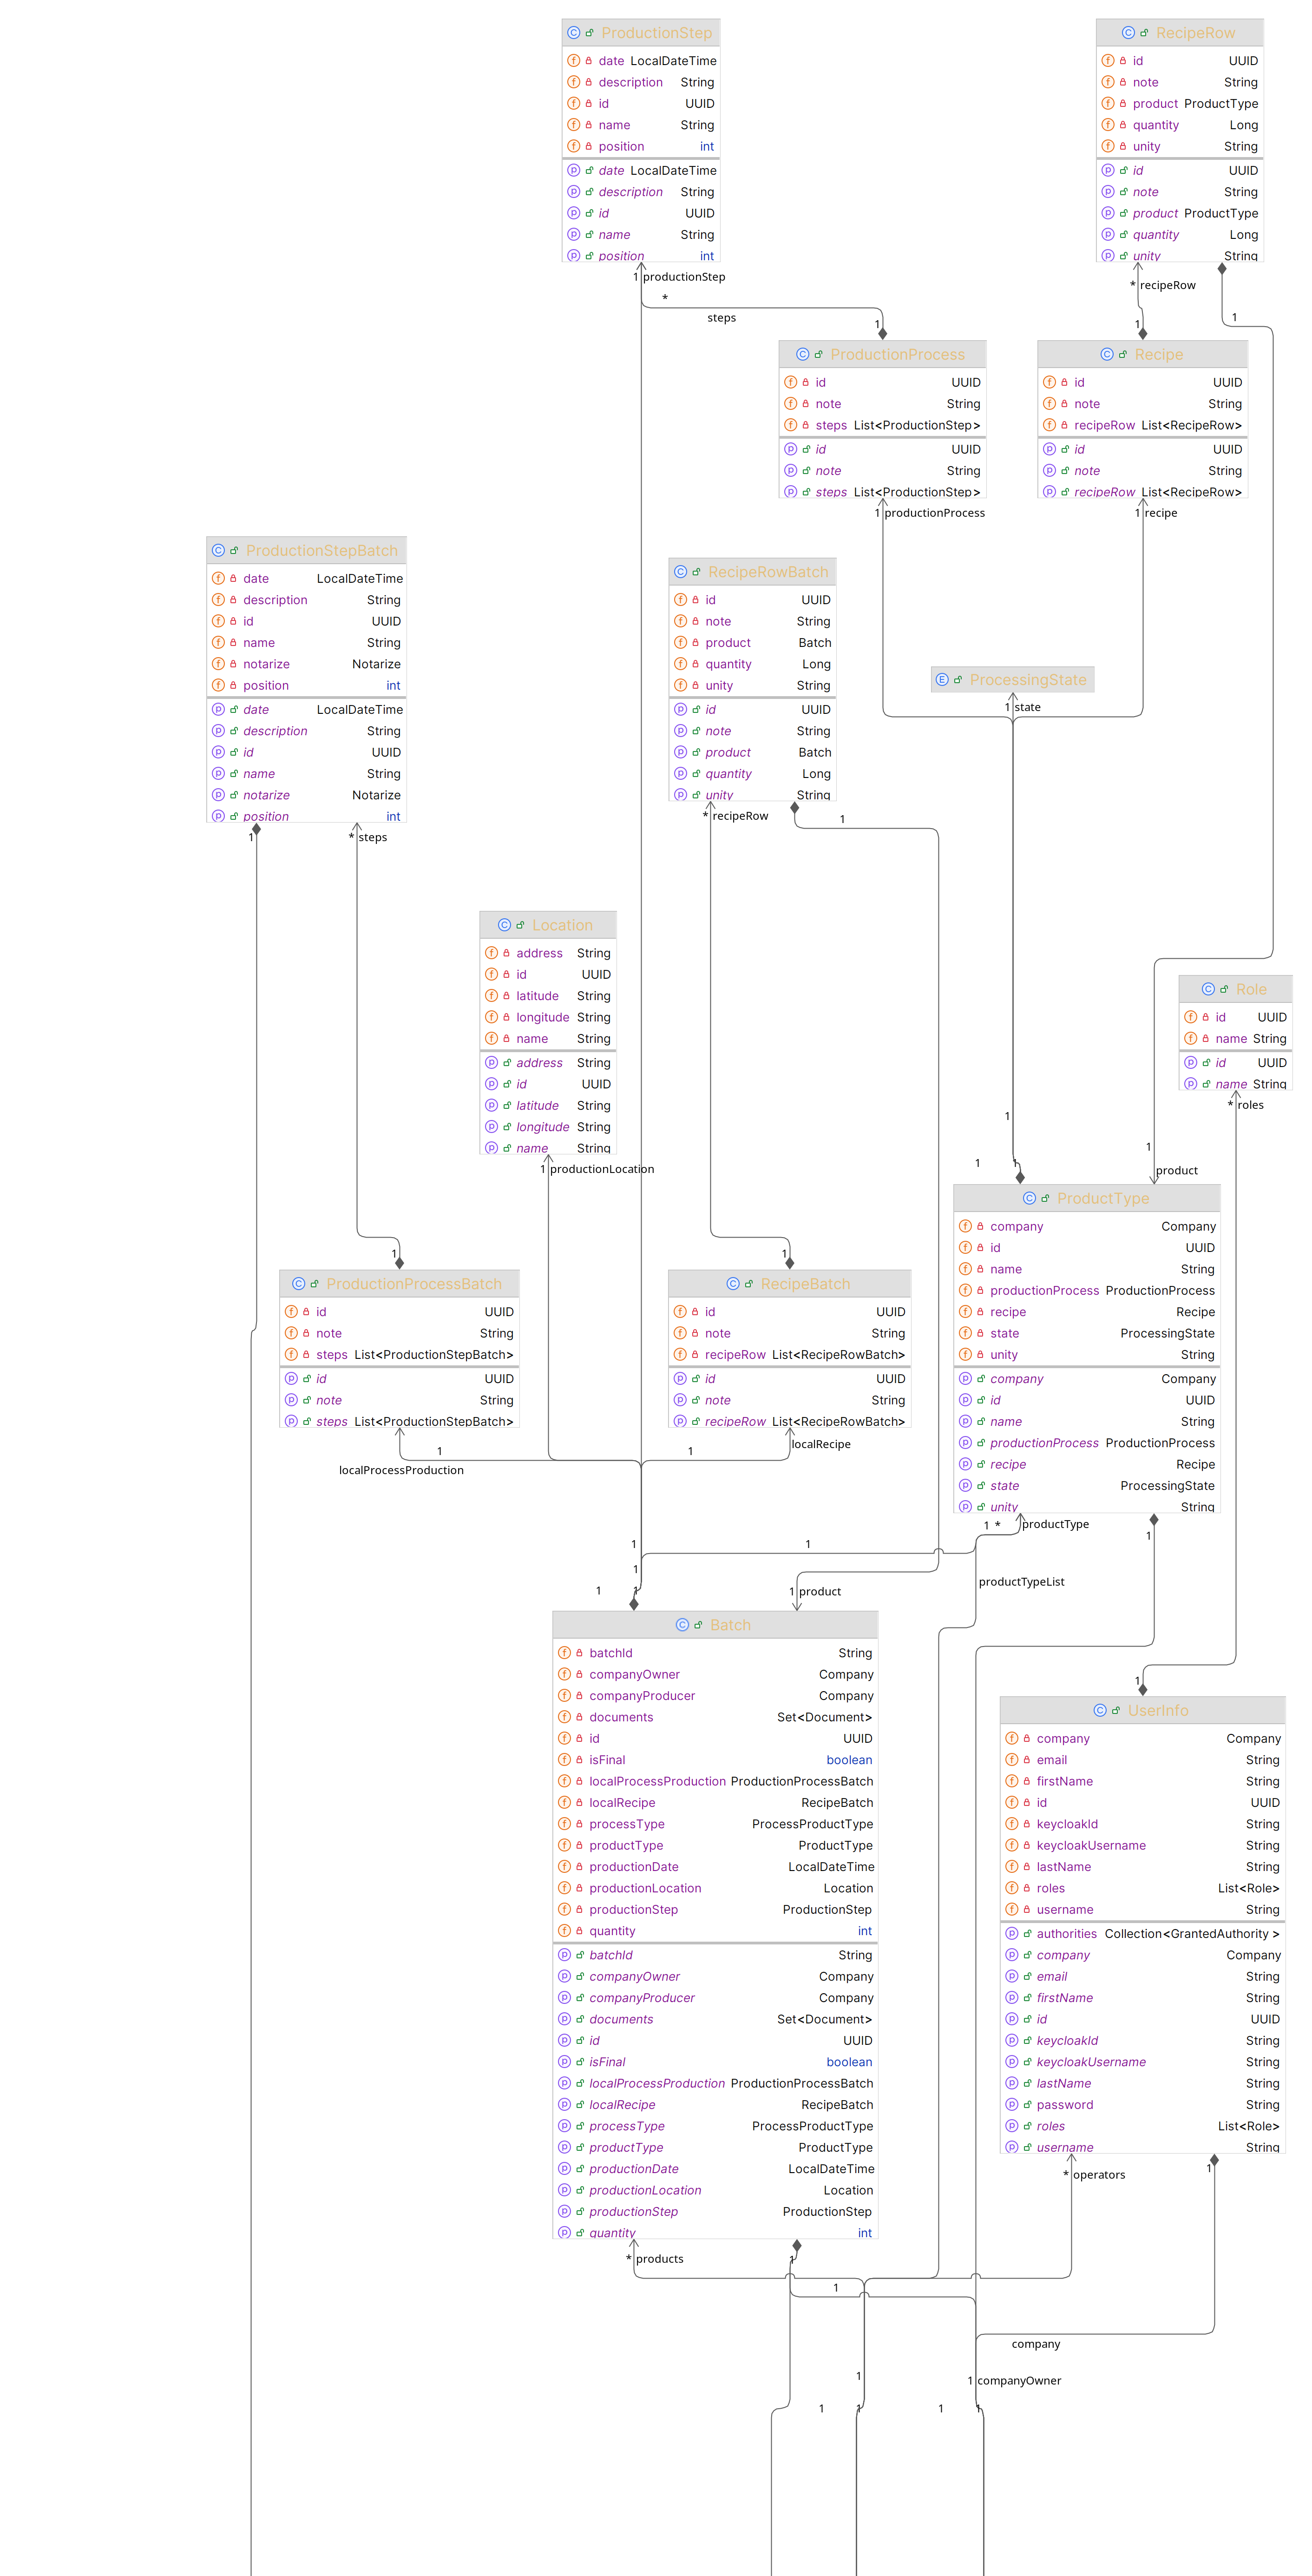
\includegraphics[height=20cm]{img/model3_up.png}
  \caption{Diagramma UML classi - parte 1 di 2}
  \label{fig:schemaclassi1}
\end{figure}


\begin{figure}[H]
  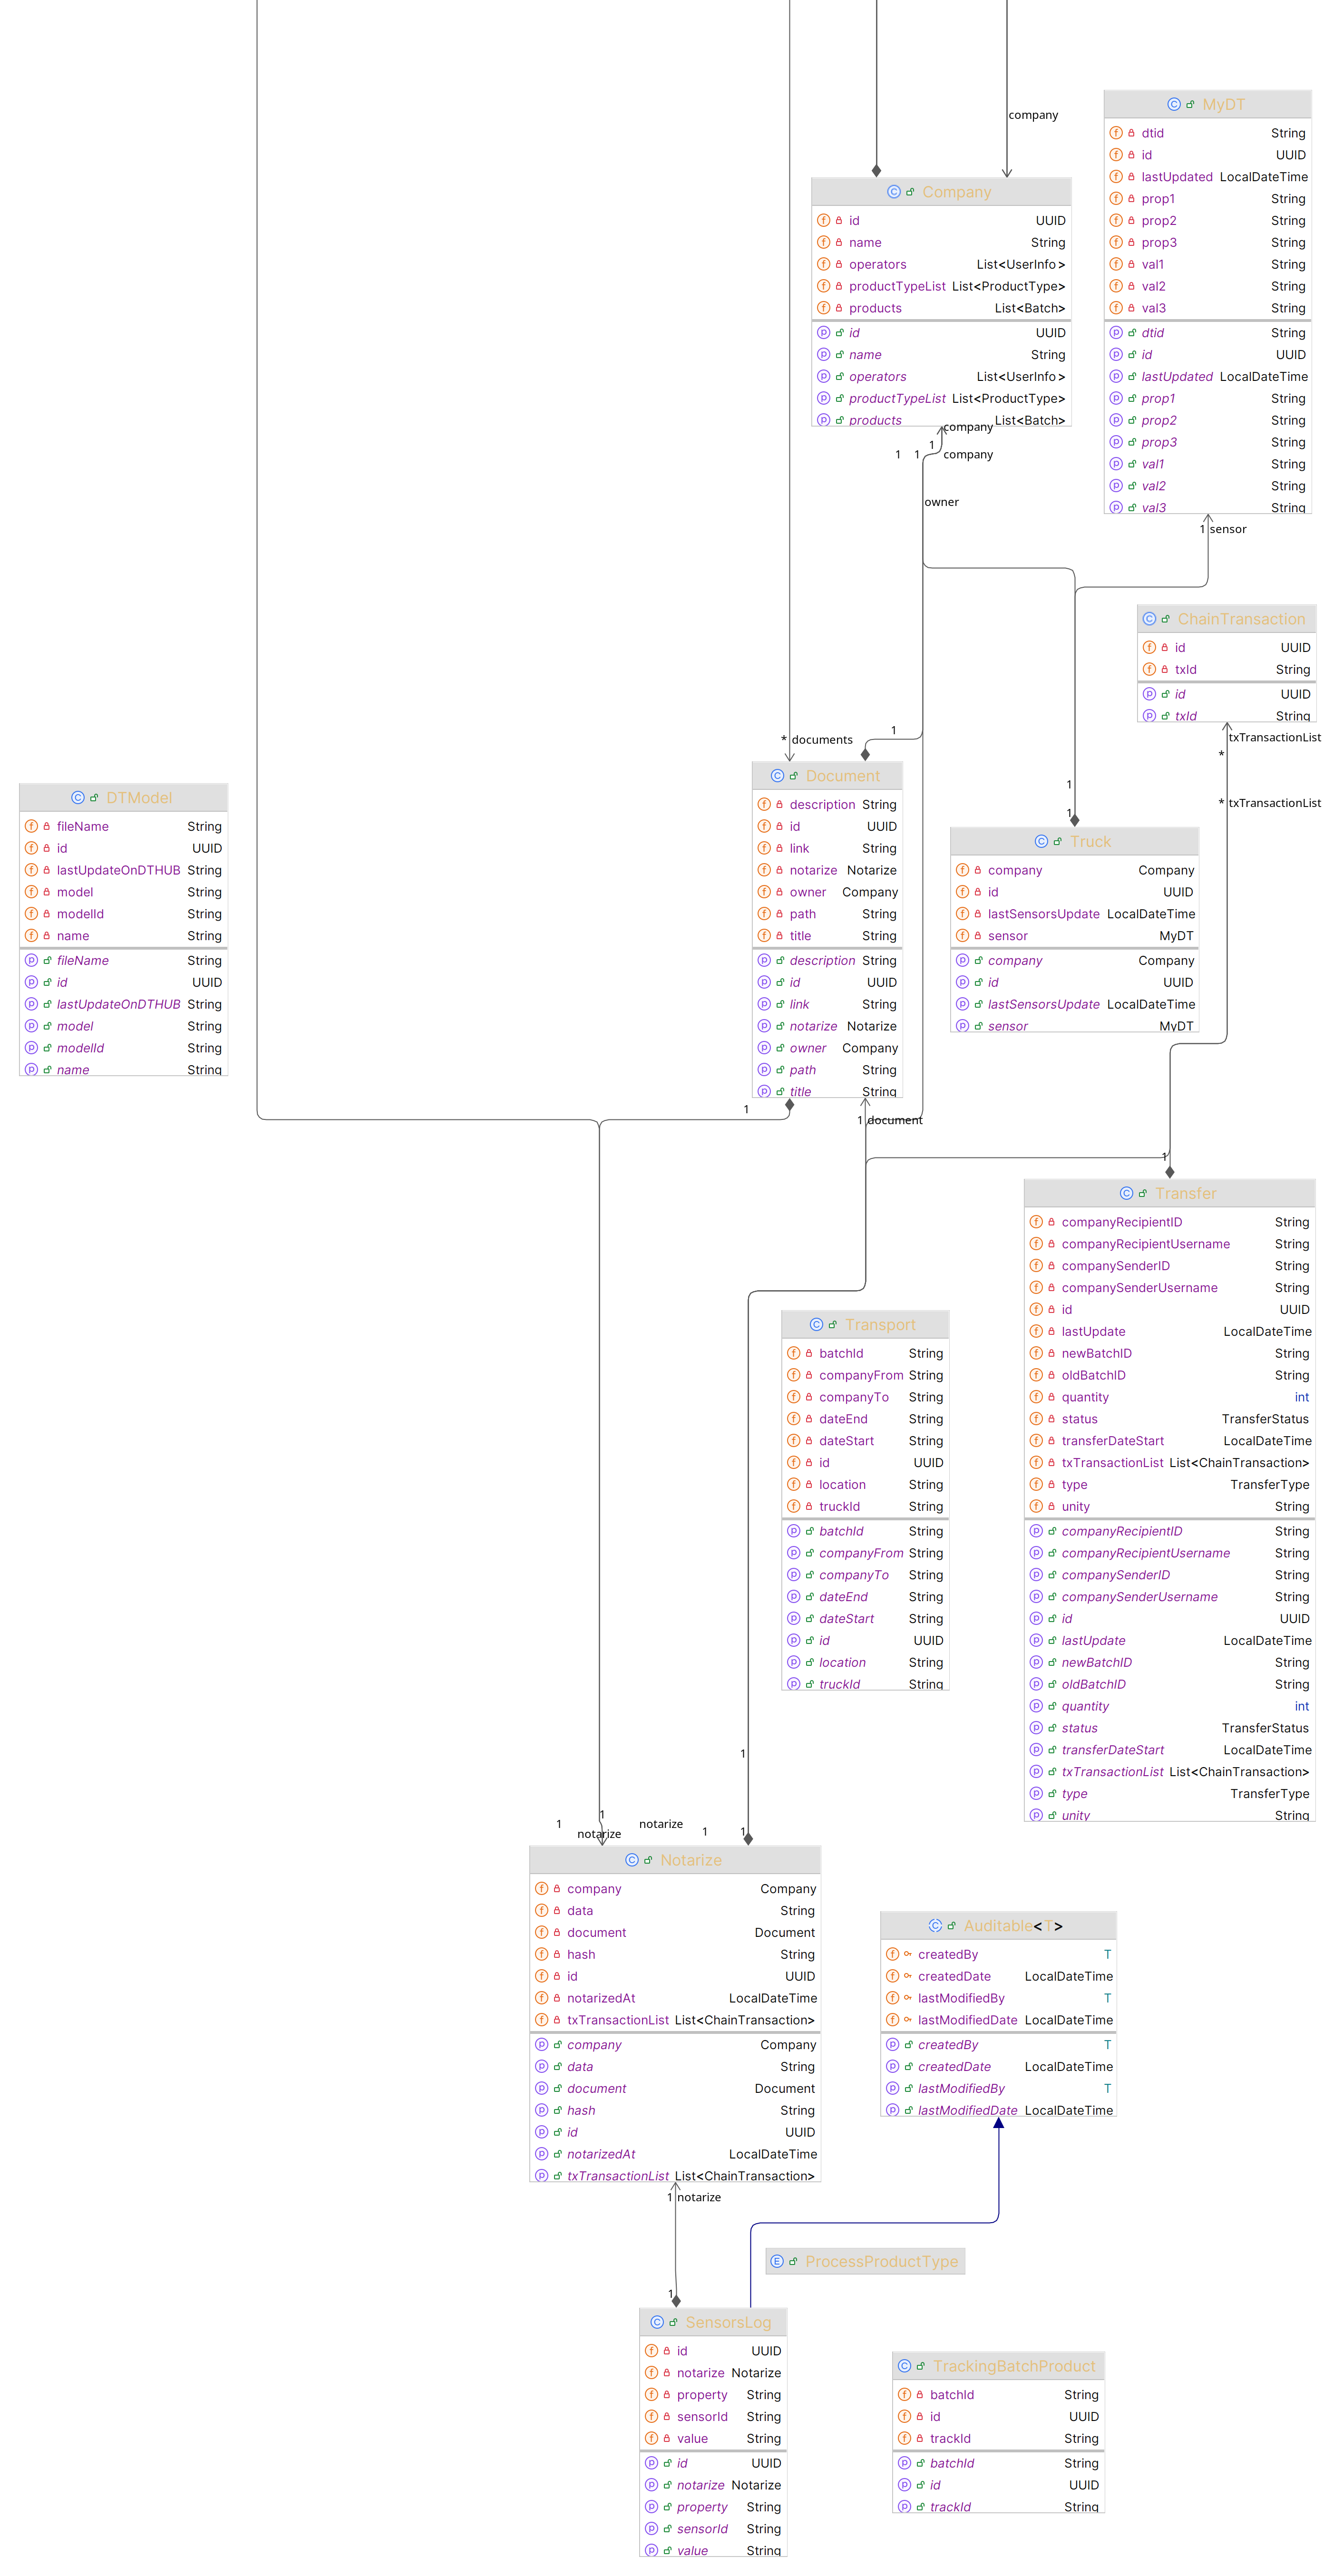
\includegraphics[height=20cm]{img/model3_down.png}
  \caption{Diagramma UML classi - parte 2 di 2}
  \label{fig:schemaclassi2}
\end{figure}

%% --------- SCHEMA ENTITA-RELAZIONE ------------------
\begin{figure}[H]
  \includegraphics[height=1\linewidth, angle=-90]{example-image-a}
  \caption{Schema Entità-Relazione}
  \label{fig:schemaer}
\end{figure}


%% --------- UML  ------------------
\begin{figure}[H]
  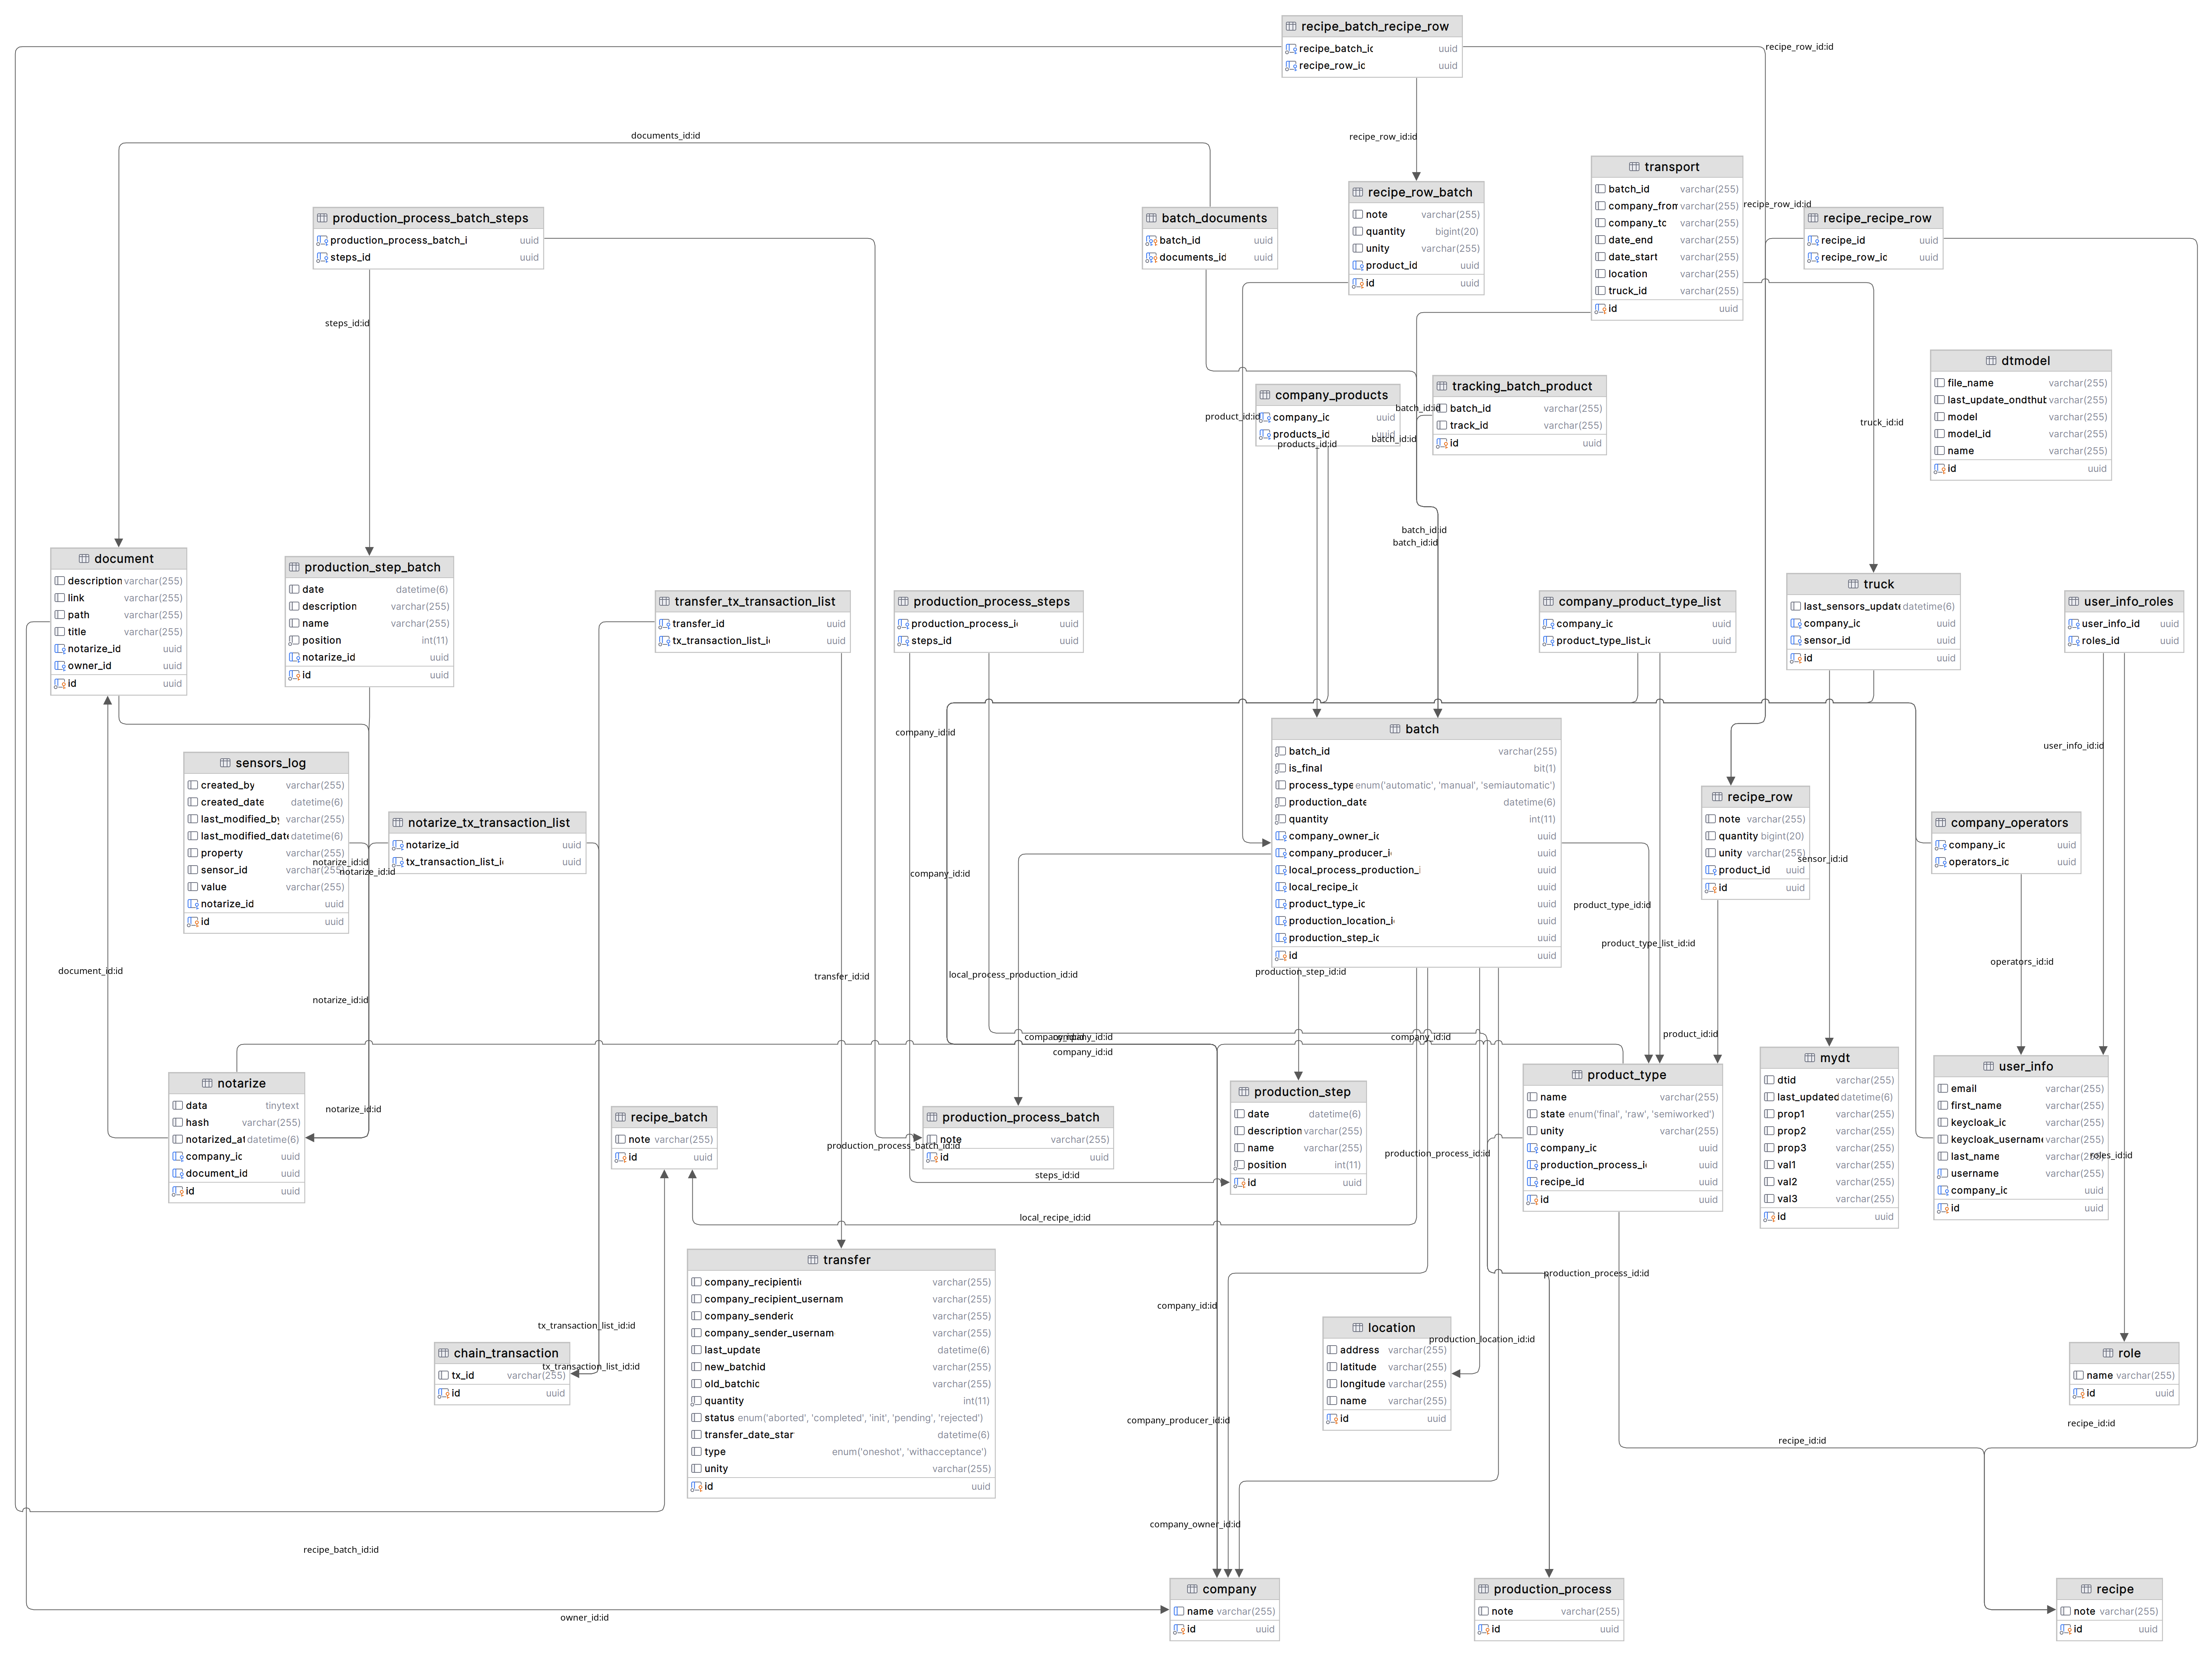
\includegraphics[height=1\linewidth, angle=-90]{img/db.png}
  \caption{Schema logico base di dati}
  \label{fig:schemauml}
\end{figure}

\subsubsection{Answar Set Programming}

Il modulo di answer set programming utilizza, tramite un wrapper non ufficiale rilasiato con licenza open source, il pacchetto clingo di Potasco \footnote{https://github.com/potassco/clingo} che rappresenta una soluzione completa all'esecuzione di programmi ASP perché combina insieme entrambe le componenti necessarie ad una esecuzione corretta di un programma ASP, ovvero il grounder gringo che il solutore clasp.

Ad un livello precedente troviamo un servizio middleware costruito ad hoc che prepara le strutture dati Java in programmi eseguibili da clingo, quindi compie un operazione di serializzazione.

L'output di clingo è poi opportunamente gestito da un altra porzione del servizio middleware che si occupa della deserializzazione della stringa che rappresenta l'output.

\subsubsection{Gemello digitale}

I gemelli digitali utilizzati nel progetto sono stati implementati sfruttando la piattaforma Digital Twin di Microsoft Azure. Questo servizio è una piattaforma a servizi (PaaS) che consente la gestione di gemelli digitali sia autonomi che eventualmente integrati con altri servizi, non necessariamente limitati al contesto Azure, poiché vengono esposti degli endpoint che, al netto di un'eventuale stretta sulle politiche di accesso definita dall'utente, sono pubblici ed implementano lo standard RESTAPI.
L'integrazione e l'utilizzo dei gemelli digitali in una applicazione Java necessita di una componente software specializzata. In questo caso ci si è diretti verso il Software Development Kit (SDK) fornito da Microsoft Azure.
L'SDK fornisce un approccio modulare consentendo l'adozione solo delle parti necessarie ed in particolare si è utilizzato il modulo "Azure IoT Digital Twins client library for Java".

\subsubsection{Smart contract e blockchain}

Gli smart contract posso essere visti come le classi di un programma orientato agli oggetti, Java ad esempio. Si possono scrivere in diversi linguaggi di programmazione, a seconda della blockchain utilizzata. In questo progetto di tesi si utilizza Polygon e gli smart contract su Polygon si scrivono in Solidity.

\quote{
  Solidity è un linguaggio di alto livello orientato agli oggetti per l'implementazione di contratti intelligenti. I contratti intelligenti sono programmi che regolano il comportamento dei conti all'interno dello stato di Ethereum. [...] è un linguaggio a parentesi graffe progettato per la macchina virtuale di Ethereum (EVM). È influenzato da C++, Python e JavaScript. [...] Solidity è tipizzato staticamente, supporta l'ereditarietà, le librerie e i tipi complessi definiti dall'utente \footnote{Tradotto con DeepL.com (versione gratuita)} \cite{soliditylangSolidityx2014}
}

Durante la fase preliminare di scouting delle librerie sono stati individuati alcuni tool di interesse. Si e' individuato il seguente stack tecnologico per la compilazione e la distribuzione di contratti scritti in Solidity ed eseguibili all'interno di una Ethereum Virtual Machine.

\begin{itemize}
  \item \textbf{Solidity} scrittura del contratto
  \item \textbf{HardHat} compilazione, distribuzione e test dei contratti
  \item \textbf{Ether.js} client Ethereum per NodeJS
\end{itemize}

Inoltre affinché la piattaforma supporti pienamente le operazioni di lettura e scrittura su un registro distribuito è necessario utilizzare alcuni componenti software aggiuntivi. Nello stack tecnlogico adottato è possibile inserire a questo proposito il progetto Web3j, una libreria java che supporta gli SmartContract e consente di interagire con la rete Etherium tramite un client JSON-RPC, utilizzando chiamate API su protocollo HTTP o IPC. \cite{web3jQuickstartWeb3j}

\begin{figure}[H]
  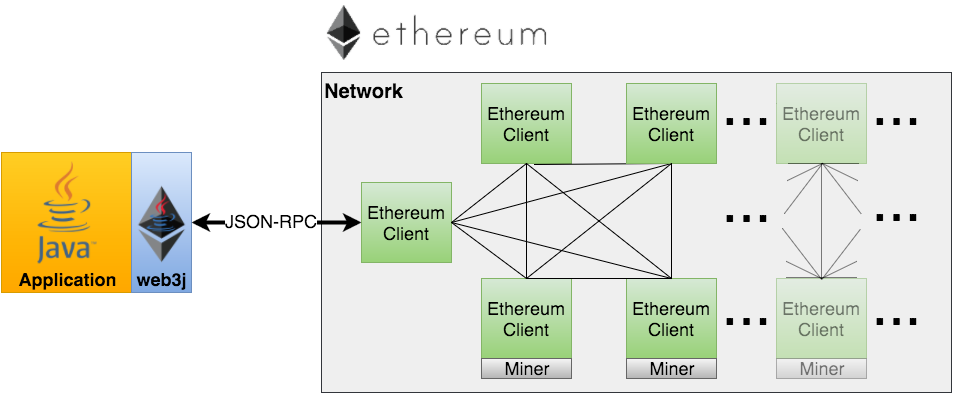
\includegraphics[width=1\linewidth]{img/image-2.png}
  \caption{Web3j \cite{web3jQuickstartWeb3j}}
  \label{fig:web3j}
\end{figure}

Essendo Java un linguaggio fortemente tipizzato necessita di un tipo, di una classe, che rappresenti lo smart contract per poter essere utilizzato all'interno dell'applicazione. La libreria offre un tool a riga di comando che consente la generazione automatica di un wrapper, una classe java, per ogni contratto scritto in solidity che si vuole utilizzare.

Benché Web3j supporti ogni aspetto del ciclo di vita degli smart contract, si è deciso di adottare una soluzione software differenze per la distribuzione, il testing e la verifica dei contratti, creando di fatto un modulo separato e isolato dal resto dell'applicazione e lasciando alla parte Spring-Web3j solo la responsabilità dell'utilizzo vero e proprio dei contratti.

Il modulo di creazione dei contratti risiede in ambiente NodeJS ed utilizza il framework HardHat.js.

Hardhat è un framework modulare composto da diverse parti tra loro interconnesse ma comunque autonome. Nella documentazione del progetto si definisce il framework come un ambiente di sviluppo. Hardhat is a development environment for Ethereum software. It consists of different components for editing, compiling, debugging and deploying your smart contracts and dApps, all of which work together to create a complete development environment. \cite{hardhatGettingStarted}

Le parti principali che compongono l'ambiente di sviluppo sono:

\begin{itemize}
  \item runner: è il componente principale di hardhat, consente di compilare, distribuire, testare e verificare gli smart contract
  \item ignition: consente di utilizzare un approccio dichiarativo alla gestione degli smart contract
  \item net: una rete locale di test
  \item estensione per visual studio code
\end{itemize}

Degna di nota è sicuramente la parte di testing degli smart contract che attraverso l'integrazione di librerie ben note in ambito Test Drive Development (TDD)su NodeJs quali Mocha \footnote{https://mochajs.org/} e Chai \footnote{https://www.chaijs.com/} consente un rapido sviluppo di smart contract sicuri e testati.
I contratti utilizzati in piattaforma sono stati sviluppati seguendo un approccio TDD, raggiungendo un valore di coverage superiore al 90%.

Una delle motivazioni principali che hanno spinto verso questa scelta di separazione è stata il pieno supporto di questo altro stack tecnologico alla libreria OpenZeppelin, la cui adozione riveste un'importante scelta in ambito di sicurezza degli smart contract. Basti pensare che uno smart contract che non adotta strategie difensive di alcun tipo può essere utilizzato da chiunque ne conosca l'indirizzo (pubblico!). Questo sicuramente non è un comportamento voluto o desiderato dalla maggior parte dei contesti applicativi. Un primo rimedio che offre OpenZeppelin è la super classe Owanable che se implementata consente di porre vincoli sull'utente che può effettivamente utilizzare il contratto, anche se ne conosce l'indirizzo. Esistono livelli più avanzati di gestione degli accessi e dei ruoli ed OpenZeppelin offre supporto anche a questi casi d'uso.

\subsubsection{Riflessioni sulla sicurezza degli smart contract}

\begin{longlisting}
  \inputminted{solidity}{./code/Hash.v2.sol}
  \caption{Contratto di notarizzazione - versione finale}
  \label{listing:hash2}
\end{longlisting}

% Open zeppelin
% tipi di attacchi ed eventuali vulnerabilità

\subsection{Implementazione - server side}

Sono state effettuate delle scelte a livello implementativo.
- Ultima versione Java attualmente disponibile (22) in versione OpenJDK.
- Utilizzo di Keycloak in versione dockerizzata


\subsubsection{Autenticazione}
L'autenticazione degli utenti è gestita dal server autoritativo Keycloak. In un contesto OAuth2 il componente Spring riveste il ruolo di resource server, Keycloak è l'authentication server, le risorse sono le informazioni veicolate tramite le chiamate alle API\footnote{Application Programming Interface - per una lista degli endpoints disponibili vedere ?? } ed in fine la componente d'interfaccia, che viene eseguita nel browser dell'utente, è il client.

\begin{figure}[H]
  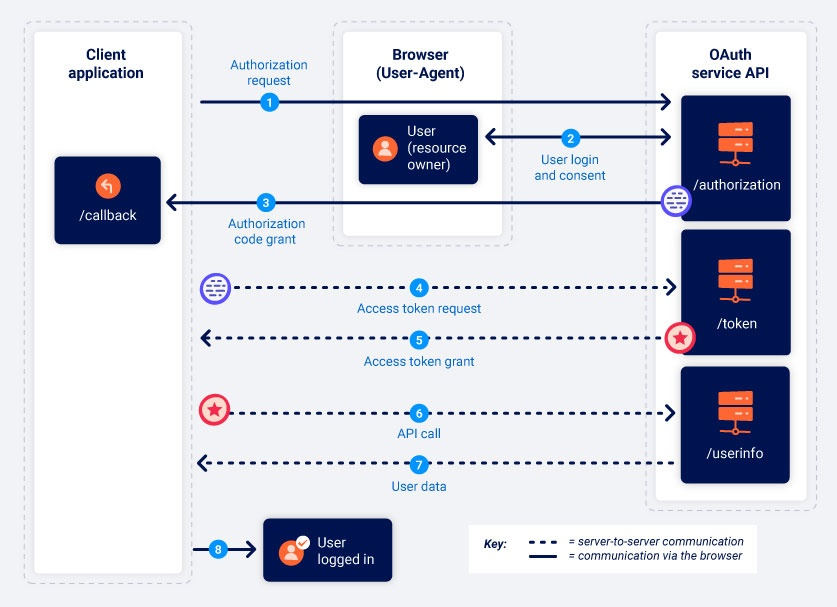
\includegraphics[width=1\linewidth]{img/oauth-authorization-code-flow.jpg}
  \caption{Authorization code grant type - da \cite{portswiggerOAuthGrant}}
  \label{fig:flussoportswigger}
\end{figure}

Keycloak è implementato utilizzando la tecnologia di conteinerizzazione Docker. I docker sono container definiti leggeri poiché l'isolamento che offrono riguarda i processi. In una macchina virtuale, definita conteinerizzazione pesante, il grado di isolamento è maggiore, visto che si instanzia un sistema operativo da zero e la condivisione tra sistema operativo ospitante (host) e sistema operativo emulato (guest) è limitata alle risorse hardware. Con le macchine virtuali si massimizza l'isolamento ma si massimizza anche l'overhead inteso come dispendio di energie computazionali spese nella gestione di elementi \textit{duplicati}, altrimenti già disponibili nel sistema host. \cite{dockerWhatContainer}

In questo contesto prototipale, il server autoritativo è stato avviato in modalità di sviluppo. Le limitazioni e le semplificazioni apportate riguardano la gestione del TLS e della mutua autenticazione. In fase di sviluppo non è richiesta la configurazione di un keystore java.

\begin{listing}
  \inputminted{shell}{./code/avvio.kc.sh}
  \caption{Keycloak - Comando di avvio}
  \label{listing:avviokc}
\end{listing}

Il comando di avvio utilizzato è una personalizzazione del comando che si può trovare nella documentazione ufficiale \cite{keycloakDockerKeycloak}. L'adattamento effettuato serve a caricare all'avvio il file di configurazione di progetto. Nel file di configurazione sono esplicitati tutte le impostazioni di \textit{realm}. Il realm è l'ambito di autenticazione, lo scope per dirla in termini strettamente di codice, per cui quando un utente si registra o viene creato esso è registrato o creato all'interno di un realm. In questo caso la piattaforma ha un suo realm. Il resource server e il client, rispettivamente componente Spring e componente Angular, sono registrati sul server autoritativo come client del ream \textit{iotchain}.

\subsubsection{Application Programming Interface (API)}

Sono state definite i senguenti endpoints:

\begin{itemize}
  \item \texttt{GET /api/v1/company/batch}
    \\ Descrizione:
    \\ Tipo di accesso:
    \\ Input:
    \\ Output:

  \item \texttt{POST /api/v1/company/batch}
    \\ Descrizione:
    \\ Tipo di accesso:
    \\ Input:
    \\ Output:

  \item \texttt{GET /api/v1/company/batch/{{id}}}
    \\ Descrizione:
    \\ Tipo di accesso:
    \\ Input:
    \\ Output:

  \item \texttt{GET /api/v1/company/batch/{{id}}/track}
    \\ Descrizione:
    \\ Tipo di accesso:
    \\ Input:
    \\ Output:

  \item \texttt{GET /api/v1/company/product-type}
    \\ Descrizione:
    \\ Tipo di accesso:
    \\ Input:
    \\ Output:

  \item \texttt{POST /api/v1/company/product-type}
    \\ Descrizione:
    \\ Tipo di accesso:
    \\ Input:
    \\ Output:

  \item \texttt{GET /api/v1/company/client}
    \\ Descrizione:
    \\ Tipo di accesso:
    \\ Input:
    \\ Output:

  \item \texttt{GET /api/v1/company/transfer}
    \\ Descrizione:
    \\ Tipo di accesso:
    \\ Input:
    \\ Output:

  \item \texttt{POST /api/v1/company/transfer}
    \\ Descrizione:
    \\ Tipo di accesso:
    \\ Input:
    \\ Output:

  \item \texttt{GET /api/v1/company/transfer/\{\{batch\_id\}\}}
    \\ Descrizione:
    \\ Tipo di accesso:
    \\ Input:
    \\ Output:

  \item \texttt{GET /api/v1/company/transfer/\{\{trans\_id\}\}/abort}
    \\ Descrizione:
    \\ Tipo di accesso:
    \\ Input:
    \\ Output:

  \item \texttt{GET /api/v1/company/transfer/\{\{trans\_id\}\}/accept}
    \\ Descrizione:
    \\ Tipo di accesso:
    \\ Input:
    \\ Output:

  \item \texttt{GET /api/v1/company/transfer/\{\{trans\_id\}\}/reject}
    \\ Descrizione:
    \\ Tipo di accesso:
    \\ Input:
    \\ Output:

  \item \texttt{GET /api/v1/company/doc}
    \\ Descrizione:
    \\ Tipo di accesso:
    \\ Input:
    \\ Output:

  \item \texttt{GET /api/v1/company/doc/notarize/\{\{doc\_id\}\}}
    \\ Descrizione:
    \\ Tipo di accesso:
    \\ Input:
    \\ Output:

  \item \texttt{POST /api/v1/company/doc/upload}
    \\ Descrizione:
    \\ Tipo di accesso:
    \\ Input:
    \\ Output:

  \item \texttt{GET /api/v1/company/doc/\{\{doc\_id\}\}}
    \\ Descrizione:
    \\ Tipo di accesso:
    \\ Input:
    \\ Output:

  \item \texttt{GET /api/v1/company/doc/\{\{doc\_id\}\}/resource}
    \\ Descrizione:
    \\ Tipo di accesso:
    \\ Input:
    \\ Output:

  \item \texttt{POST /api/v1/public/doc/check/{{hash}}}
    \\ Descrizione:
    \\ Tipo di accesso:
    \\ Input:
    \\ Output:

  \item \texttt{GET /api/v1/company/transport}
    \\ Descrizione:
    \\ Tipo di accesso:
    \\ Input:
    \\ Output:

  \item \texttt{POST /api/v1/company/transport}
    \\ Descrizione:
    \\ Tipo di accesso:
    \\ Input:
    \\ Output:

  \item \texttt{GET /api/v1/company/transport/\{\{batch\_id\}\}}
    \\ Descrizione:
    \\ Tipo di accesso:
    \\ Input:
    \\ Output:

  \item \texttt{GET /api/v1/company/transport/\{\{transport\_id\}\}/truck}
    \\ Descrizione:
    \\ Tipo di accesso:
    \\ Input:
    \\ Output:

  \item \texttt{GET /api/v1/company/truck}
    \\ Descrizione:
    \\ Tipo di accesso:
    \\ Input:
    \\ Output:

  \item \texttt{GET /api/v1/company/truck/update}
    \\ Descrizione:
    \\ Tipo di accesso:
    \\ Input:
    \\ Output:

  \item \texttt{GET /api/v1/company/notarization}
    \\ Descrizione:
    \\ Tipo di accesso:
    \\ Input:
    \\ Output:

  \item \texttt{POST /api/v1/company/notarization/step/\{\{step\_id\}\}}
    \\ Descrizione:
    \\ Tipo di accesso:
    \\ Input:
    \\ Output:

\end{itemize}

\subsubsection{Persistenza}

L'implementazione della persistenza da un punto di vista fisico e di basso livello è stata demandata all'ORM (Object Relational Mapping) utilizzato, Hibernate, nella versione XXX. Il DBMS usato in questa fase prototipale è MariaDB 11.4.2 installato in modo nativo sulla macchina di sviluppo (quindi non conteinerizzato).

Per ogni concetto evidenziato in \ref{modellodominio} è stata creata una classe Java marcata come entità usando l'annotazione \texttt{@Entity} del layer di persistenza di Jakarta (specifica implementata da Hibernate).

Ogni entità del modello di dominio estende la classe astratta \texttt{Auditable} così da permettere un tracciamento dettagliato delle modifiche alle entità stesse.
Ogni entità utilizza come chiave primaria un identificativo univoco di tipo alfanumerico, uno Universally unique identifier (UUID). Gli UUID posso essere di diversi tipi, il tipo utilizzato è il tipo 4, il tipo randomico. Questo tipo di dato è utilizzabile in maniera nativa perché MariaDB dalla versione 10.7 \cite{mariadbUUIDData} supporta nativamente il tipo UUID.


\subsubsection{Programmazione Asincrona e thread virtuali}
Il server implementato è un server che ha un funzionamento sincrono e bloccante. Ovvero il sistema riceve e gestisce la connessione in ingresso e su di questa si blocca, attendendo l'esito della computazione prima di chiudere la connessione stessa. In un contesto simile è complesso gestire la comunicazione con la blockchain o con altri servizi quali la piattaforma di gestione dei digital twin. Si è rivelato indispensabile attivare la possibilità di effettuare chiamate asincrone che funzionano in un ottica multithread: la connessione in ingresso è gestita e chiusa dall'application server (Tomcat) quasi immediatamente, senza dover attendere il termine della chiamata asincrona. La chiamata a funzione asincrona esegue la computazione e poi salva il risultato della computazione stessa sulla base di dati, rendendo persistente l'informazione. Eliminando di fatto la necessità per l'utente di attendere il termine della connessione che durante alcuni test di scrittura sulla chain, con rete sovraffollata, può superare i 10 minuti di attesa. Il risultato della scrittura sulla blockchain quando disponibile si può ottenere effettuando una semplice interrogazione sulla base di dati. Per una migliore gestione delle risorse sono stati utilizzati i thread virtuali, che la JVM mette a disposizione degli sviluppatori a partire dalla versione 21. I thread virtuali, a differenza dei thread di sistema, sono gestiti dalla JVM e non richiedono chiamate di sistema. Offro il vantaggio di poter essere sospesi dalla JVM e liberare il thread di sistema sottostante,  quando per esempio si compiono operazioni I/O bloccanti, ed essere ripresi quando è possibile. Il thread di sistema liberato può eseguire altri thread virtuali. \cite{oraclevirtualthread}

La configurazione utilizzata in piattaforma è la seguente:


\begin{longlisting}
  \inputminted{java}{./code/async.spring.java}
  \caption{Configurazione Asincrona da \cite{baeldungWorkingWith}}
  \label{listing:asyncconfig}
\end{longlisting}

Una funzione annotata come \texttt{@Bean} consente di utilizzate la funzione stessa in ogni porzione di codice, utilizzando la dependency injection e l'inversione del controllo forniti da Spring.
Questi due Bean di configurazione specificano quale tipologia di Thread si vuole utilizzare, con il Tomcat fornito da Spring Boot e con le funzioni annotate come asincrone.
I thread virtuali offrono prestazioni nettamente migliori in termini di richieste gestite nell'unità di tempo \cite{baeldungWorkingWith}.

\subsubsection{Answer Set Programming}

Per poter utilizzare all'interno di un contesto più ampio un programma in AnswareSetProgramming (ASP) che sia dinamico, ovvero che utilizzi dati che cambiano nel tempo e provengono da computazioni effettuate in altri moduli del software, è necessario in un primo momento effettuare una mappatura della struttura dati in input al programma stesso e successivamente a comp

\begin{longlisting}
  \inputminted{prolog}{./code/checkBatchInput.lp}
  \caption{Programma ASP - Ricerca lotto - Esempio fatti in input}
  \label{listing:asp1}
\end{longlisting}


\begin{longlisting}
  \inputminted{prolog}{./code/checkBatch.lp}
  \caption{Programma ASP - Ricerca lotto}
  \label{listing:asp2}
\end{longlisting}

\begin{longlisting}
  \inputminted{java}{./code/asp.mapinput.java}
  \caption{ASP - Mapping in ingresso}
  \label{listing:asp3}
\end{longlisting}


\begin{longlisting}
  \inputminted{java}{./code/asp.mapout.java}
  \caption{ASP - Mapping in uscita}
  \label{listing:asp4}
\end{longlisting}

\begin{longlisting}
  \inputminted{java}{./code/asp.solve.java}
  \caption{ASP - Solutore}
  \label{listing:asp5}
\end{longlisting}

\subsubsection{Gemello digitale}

\begin{longlisting}
  \inputminted{json}{./code/Truck.json}
  \caption{Modello di Gemello Digitale implementato}
  \label{listing:dt0}
\end{longlisting}

\begin{longlisting}
  \inputminted{java}{./code/Truck.json}
  \caption{Modello di Gemello Digitale implementato}
  \label{listing:dt1}
\end{longlisting}


\begin{longlisting}
  \inputminted{java}{./code/dt.create.java}
  \caption{Creazione del gemello digitale}
  \label{listing:dt2}
\end{longlisting}


\begin{longlisting}
  \inputminted{java}{./code/dt.init.java}
  \caption{Creazione del gemello digitale}
  \label{listing:dt3}
\end{longlisting}

\begin{longlisting}
  \inputminted{java}{./code/dt.polling.java}
  \caption{Creazione del gemello digitale}
  \label{listing:dt4}
\end{longlisting}

\begin{longlisting}
  \inputminted{java}{./code/dt.update.java}
  \caption{Creazione del gemello digitale}
  \label{listing:dt5}
\end{longlisting}

\begin{figure}[H]
  \centering
  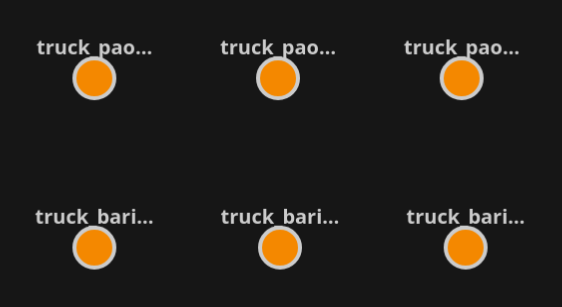
\includegraphics[width=0.5\linewidth]{img/dt_explorer.png}
  \caption{Visualizzazione dei gemelli digitali creati utilizzando il software Azure Digital Twin Explorer }
  \label{fig:azureexplorer}
\end{figure}

\subsubsection{Smart contract}

Lo smart contract con funzione di notarizzazione è stato da prima costruito come si vede nel listato \ref{listing:hash1}.

\begin{listing}[H]
  \inputminted{solidity}{./code/Hash.v1.sol}
  \caption{Contratto di notarizzazione - versione iniziale}
  \label{listing:hash1}
\end{listing}

Durante la fase preliminare di scouting delle librerie sono stati individuati alcuni tool di interesse. Si è individuato il seguente stack tecnologico per la compilazione e la distribuzione di contratti scritti in Solidity ed eseguibili all'interno di una Ethereum Virtual Machine.

\begin{itemize}
  \item \textbf{Solidity} scrittura del contratto
  \item \textbf{HardHat.js} compilazione, distribuzione e test dei contratti
  \item \textbf{Ether.js} client Ethereum per NodeJS
\end{itemize}



\begin{longlisting}[H]
  \inputminted{typescript}{./code/hardhat.config.ts}
  \caption{HardHat Configurazione}
  \label{listing:hardhatconf}
\end{longlisting}

\begin{longlisting}[H]
  \inputminted{typescript}{./code/hash.deploy.ts}
  \caption{Script per la distribuzione del contratto Hash}
  \label{listing:hash4}
\end{longlisting}

\begin{longlisting}[H]
  \inputminted{typescript}{./code/hash.listener.ts}
  \caption{Script per l'utilizzo del contratto Hash - Observer}
  \label{listing:hash5}
\end{longlisting}

\begin{longlisting}[H]
  \inputminted{typescript}{./code/hash.sign.ts}
  \caption{Script per l'utilizzo del contratto Hash - Signer}
  \label{listing:hash6}
\end{longlisting}


\subsection{Implementazione - interfaccia}


\section{Risultati e conclusioni}

\clearpage
\section{Riferimenti}
\listoffigures
\clearpage
\listoftables
\clearpage
\renewcommand\listoflistingscaption{Elenco del codice sorgente}
\listoflistings % Now typeset the list
\clearpage
\printbibliography
\end{document}
